\documentclass[letterpaper,twocolumn,10pt]{article}

\usepackage{algorithmicx}
\usepackage{wrapfig}
\usepackage{algorithm}
\usepackage{algpseudocode}
\usepackage{amsmath}
\usepackage{bm}
\usepackage{calc}
\usepackage{lipsum}
\usepackage{pervasives}
\usepackage{subcaption}
\usepackage{tikz}
\usepackage{usenix2019_v3}
\usetikzlibrary{calc}
\usetikzlibrary{positioning}

\newcommand{\deps}[1]{\text{deps}}
\newcommand{\msg}[1]{\langle #1 \rangle}
\newcommand{\leadercolor}{flatblue}
\newcommand{\proposercolor}{flatpurple}
\newcommand{\replicacolor}{flatred}
\newcommand{\clientcolor}{white}
\newcommand{\depservicecolor}{flatgreenalt}
\newcommand{\consensuscolor}{flatbrown}

% Remove the "end if" from algorithmicx. See [1].
%
% [1]: https://tex.stackexchange.com/a/53518
\algtext*{EndIf}
\algtext*{EndFor}

% Custom upon ... do block.
\algblockdefx[Upon]{Upon}{EndUpon}
  [1]{\textbf{upon} #1 \textbf{do}}
  {end}
\algtext*{EndUpon}

% Custom State: block.
\algnewcommand{\algorithmicstate}{\textbf{State:}}
\algnewcommand{\GlobalState}{\item[\algorithmicstate]}

\begin{document}
\date{}

\title{TODO}

\author{%
{\rm Michael Whittaker}\\
UC Berkeley
\and
{\rm Neil Giridharan}\\
UC Berkeley
\and
{\rm Adriana Szekeres}\\
University of Washington
\and
{\rm Joseph M. Hellerstein}\\
UC Berkeley
\and
{\rm Ion Stoica}\\
UC Berkeley
}

\maketitle

{\begin{abstract}
  In this paper, we present a family of state machine replication protocols
  inspired by Fast Paxos~\cite{lamport2006fast}, EPaxos~\cite{moraru2013there},
  and Caesar~\cite{arun2017speeding}. The protocols are called Bipartisan
  Paxos, Unanimous Bipartisan Paxos, and Majority Commit Bipartisan Paxos.
\end{abstract}

}
{\section{Introduction}
State machine replication protocols like MultiPaxos~\cite{lamport1998part,
lamport2001paxos} and Raft~\cite{ongaro2014search} allow a state machine to be
executed in unison across a number of machines, despite the possibility of
faults. Today, state machine replication is pervasive. Nearly every strongly
consistent distributed system is implemented with some form of state machine
replication~\cite{corbett2013spanner, thomson2012calvin, hunt2010zookeeper,
burrows2006chubby, baker2011megastore, cockroach2019website, cosmos2019website,
tidb2019website, yugabyte2019website}.

MultiPaxos is one of the oldest and one of the most widely used state machine
replication protocols. Despite its popularity, MultiPaxos doesn't have optimal
throughput or optimal latency. In MultiPaxos, \emph{every} command is sent to a
single elected leader. This leader becomes a bottleneck, limiting the
throughput of the protocol. Moreover, when a client sends a command to the
leader, it must wait at least two round trips before receiving a response. This
is twice as long as the theoretical minimum of one round
trip~\cite{lamport2006lower}.

An enormous number of state machine replication protocols have been proposed to
address MultiPaxos' suboptimal performance. These protocols use sophisticated
techniques that increase MultiPaxos' throughput, decrease its latency,
or both. For example, techniques like
  deploying multiple leaders~\cite{mao2008mencius, moraru2013there,
  arun2017speeding},
  %
  using flexible quorum sizes~\cite{howard2016flexible, nawab2018dpaxos}, and
  %
  separating the control path from the data path~\cite{biely2012s}
increase MultiPaxos' throughput. Techniques like
  bypassing the leader~\cite{lamport2006fast, ports2015designing, li2016just}
  and
  %
  speculatively executing commands~\cite{ports2015designing, li2016just,
  park2019exploiting}
decrease MultiPaxos' latency. Techniques like
  exploiting commutativity~\cite{lamport2005generalized, moraru2013there,
  arun2017speeding, park2019exploiting}
do both.

Many of these sophisticated protocols try to \emph{simultaneously} increase
throughput and decrease latency, using a combination of the techniques
described in the previous paragraph. For example, NoPaxos ``outperforms both
latency- and throughput-optimized protocols on their respective
metrics''~\cite{li2016just}, whereas EPaxos achieves ``optimal commit latency
in the wide-area'' while ``achieving high throughput''~\cite{moraru2013there}.

Trying to increase throughput \emph{and} decrease latency is a complex
endeavor. Protocols that aim to improve \emph{both} are forced to implement
multiple of the techniques mentioned above in a single protocol. In isolation,
these techniques are challenging to implement. When superimposed, they become
even harder. The techniques have to be sewn together in subtle and intricate
ways. These protocols become increasingly complex, with different components
tightly integrated together. Eventually, it becomes difficult to understand any
single piece of a protocol without first having a strong grasp on
the protocol as a whole. Paradoxically, newcomers must first understand the
protocol before they can begin to understand it!

In this paper, we take a different approach. Instead of chasing both throughput
\emph{and} latency, \textbf{we trade off a bit of latency for modularity}. We
present Bipartisan Paxos (BPaxos), a state machine replication protocol that
sacrifices optimal latency for a modular design. BPaxos is composed of a number
of independent modules. Each module can be understood in isolation and composed
together in a straightforward way to form the protocol as a whole. BPaxos'
modular design leads to simplicity and (surprisingly) higher throughput.

% Unfortunately, these advanced techniques don't come for free. They
% significantly complicate the protocols. MultiPaxos is already notoriously
% difficult to understand~\cite{van2015paxos, ongaro2014search}, and these
% sophisticated protocols make MultiPaxos seem like a piece of cake. In fact,
% these protocols can be so complex that bugs in the protocols can go
% undiscovered for years. Generalized Paxos~\cite{lamport2005generalized} and
% Zyzyva~\cite{kotla2007zyzzyva} had bugs that went undiscovered for seven and
% ten years respectively~\cite{sutra2011fast, abraham2017revisiting}. In writing
% this paper, we discovered bugs ourselves in EPaxos~\cite{moraru2013there} and
% DPaxos~\cite{nawab2018dpaxos} six years and one year after their publications
% respectively.
% %
% \TODO[mwhittaker]{Add bugs to appendix and reference appendix.}
%
% Worse yet, the vast majority of these protocols are incomplete. Many omit
% features, like garbage collection, that are necessary to implement the
% protocols in practice. These omitted features would add even more complexity to
% the already complex protocols.
%
% In this paper, we present a new state machine replication protocol called
% Bipartisan Paxos, or BPaxos for short. BPaxos is simpler, has higher
% throughput, and is more complete than state of the art replication protocols.

\paragraph{Simplicity}
It's hard to quantify the ``complexity'' of a protocol, how hard it is for
someone to understand. But, where there's smoke there's fire, and if we look at
protocols closely enough, we start to see smoke. Generalized
Paxos~\cite{lamport2005generalized} was published in 2005. Seven years later,
someone found a bug in one of its assumptions~\cite{sutra2011fast}.
Zyzyva~\cite{kotla2007zyzzyva}, a Byzantine replication protocol, was published
in 2007. Ten years later, the authors published a paper noting that the
protocol is actually unsafe~\cite{abraham2017revisiting}. In writing this
paper, we discovered bugs ourselves in two other protocols,
EPaxos~\cite{moraru2013there} and DPaxos~\cite{nawab2018dpaxos}, which we
confirmed with the protocols' authors. These long undiscovered bugs suggest
that protocols chasing high throughput and low latency are often forced to
sacrifice simplicity.
\TODO[mwhittaker]{Add bugs to appendix and reference.}

BPaxos' modular design makes it easier to understand. Each module can be
understood and proven correct in isolation, allowing newcomers to understand
the protocol piece by piece.
% Say something about how some modules, like consensus, implement well known
% abstractions and how we can take existing protocols and plug them in. E.g.,
% we use Paxos to implement consensus. Other protocols like EPaxos and Caesar
% implement their own consensus and have to prove everything is correct.

% Most of the sophisticated state machine replication protocols try to
% simultaneously achieve high throughput \emph{and} low latency. The key insight
% that enables BPaxos' simplicity is that trading off a bit of latency can
% significantly reduce complexity. BPaxos exploits this insight to achieve
% simplicity in three ways.
% \TODO[mwhittaker]{Quantify what we mean by ``a bit of latency''.}
%
% First, \textbf{BPaxos is modular.} Many protocols couple and co-locate
% components together to decrease latency. BPaxos takes the opposite approach and
% instead decouples the protocol into a number of independent modules. Each
% module can be understood in isolation, making the protocol understandable piece
% by piece.
%
% Second, \textbf{BPaxos leverages existing protocols.} Because BPaxos is
% composed of a number of independent modules, BPaxos is able to use existing,
% well known protocols to implement some modules. This way, BPaxos avoids
% reimplementing the wheel. For example, BPaxos uses Paxos to implement a
% consensus module.
%
% Third, \textbf{BPaxos avoids fast paths.} Most sophisticated state machine
% replication protocols, starting with Fast Paxos~\cite{lamport2006fast}, have a
% fast path and a slow path. The protocols optimistically attempt to take the
% fast path, but are sometimes forced to revert to the slow path.  Fast paths
% decrease latency in the best case but complicate parts of the protocols (e.g.,
% the recovery procedure). BPaxos does not use fast paths, again sacrificing
% latency for simplicity.

\paragraph{High Throughput}
We initially modularized BPaxos to trade off latency for simplicity.
Surprisingly, we found that modularizing the protocol also led to high
throughput. Many existing protocols pack a handful of logical processes onto a
single physical process. For example, a single process may play the role of a
Paxos proposer, acceptor, and state machine replica. This co-location leads to
lower latency. Messages sent between logical nodes do not have to traverse the
network if the two nodes are physically co-located.

BPaxos does \emph{not} couple logical processes together. Instead, we found
that by decoupling the protocol, we are able to significantly increase the
protocol's throughput using a simple trick: scaling. We perform a bottleneck
analysis on the protocol's components. Once we identify the bottleneck
component, we simply scale up the component until it is no longer the
bottleneck.

For example, if our protocol consisted of proposers, acceptors, and state
machine replicas and if we concluded that the proposers were the bottleneck, we
would simply add more proposers. This straightforward scaling is not so easy to
do in tightly coupled protocols. If every node is a proposer, an acceptor, and
a state machine replica, for example, then adding more proposers also
introduces more acceptors and more replicas. Adding more of a certain component
can actually slow down a protocol instead of speeding it up. For example, more
acceptors lead to larger quorums which lead to slower protocols.

\paragraph{Completeness}
Every node in a state machine replication protocol stores some state. For
example, MultiPaxos acceptors store a collection of votes and round numbers,
and MultiPaxos replicas store a log of state machine commands. This state grows
over time and must be garbage collected in order to avoid exhausting a
protocol's physical memory.

Garbage collection algorithms exist for protocols like MultiPaxos and Raft, but
many sophisticated state machine replication protocols are introduced without
detailing a garbage collection algorithm~\cite{%
  moraru2013there, % EPaxos
  arun2017speeding, % Caesar
  zhang2018building, % TAPIR
  mu2016consolidating % Janus
}. This leaves practitioners and protocol implementors responsible for piecing
together how to implement garbage collection correctly. Unfortunately, these
garbage collection algorithms are subtle and hard to get right. In this paper,
we detail a complete garbage collection algorithm for BPaxos. These details are
essential to implement BPaxos completely, and we believe they are also useful
to understand how to implement garbage collection in other sophisticated state
machine replication protocols.

In summary, we present the following contributions:
\begin{itemize}
  \item
    We introduce Bipartisan Paxos: a modular state machine replication protocol
    that trades off a bit of latency for a significant increase in simplicity.
  \item
    We describe how BPaxos' modularity leads to a straightforward form of
    scaling that yields high throughput without added complexity.
  \item
    We detail a garbage collection algorithm for BPaxos, a protocol that also
    sheds light on how to perform garbage collection in similar protocols.
\end{itemize}

% \begin{itemize}
%   \item consensus is important and pervasive
%   \item multipaxos is the most commonly used everywhere
%   \item multipaxos doesn't have the best throughput or latency. single master
%     means throughput bottleneck. two round trip from client not optimal either.
%   \item as a result, a ton of protocols attempting to improve on multipaxos
%     using a ton of techniques, (fast quorums, generalized, speculative exec,
%     multimaster, flexible quorum sizes, etc)
%   \item
%     multipaxos is complicated and these fancier protocols are even more complicated
%   \item Generalized, Paxos, Zyzyva, EPaxos, DPaxos all buggy
%   \item complex protocols are discouraging to implement in practice and easy to get wrong
%   \item moreover, these protocols are incomplete, leaving out essential features like gc
%   \item
%   \item in this paper, we present a new consensus protocol that is simpler than
%     state of the art, has higher throughput than state of the art, and is more
%     complete than state of the art.
%   \item
%   \item novelty 1: simplicity
%   \item --- insight 1: trade latency for simplicity
%   \item --- Paxos has a bad rep for being complicated
%   \item --- Fancier variants are even more complicated
%   \item --- modularity, re-use, no fast paths
%   \item --- emphasize not simpler than multpaxos but simpler than alternatives
%   \item novelty 2: high throughput
%   \item --- insight 2: decouple protocols leads to a huge number of benefits
%   \item --- decoupling and modularity reduce latency but improve throughput
%   \item --- decoupling helps identify throughput bottlenecks and scale the protocol
%   \item --- We can get state of the art throughput without adding complexity
%   \item novelty 3: garbage collection
%   \item --- gc is necessary. without it, processes run out of memory
%   \item --- mp has gc
%   \item --- all other protocols do not discuss it
%   \item --- gc is considerably more complex in these scenarios
%   \item --- we are the first to present gc
%   \item --- gc simplified by modular architecture
% \end{itemize}
%
%
%
%
%
%
%
%
% \begin{itemize}
%   \item Introduction
%
%   \item Background
%     \begin{itemize}
%       \item MultiPaxos
%     \end{itemize}
%
%   \item Bipartisan Paxos
%     \begin{itemize}
%       \item Main idea overview
%       \item Protocol overview with figure
%       \item Dependency service
%       \item Consensus Service
%       \item Replicas
%       \item BPaxos Nodes
%       \item Example
%       \item Full pseudo-code
%       \item Recovery
%     \end{itemize}
%
%   \item Scaling
%     \begin{itemize}
%       \item Other protocols tightly coupled
%       \item Our protocol decoupled, already gives boost
%       \item Bottleneck analysis
%       \item Scale to eliminate bottleneck
%     \end{itemize}
%
%   \item Garbage Collection
%     \begin{itemize}
%       \item Leaders
%       \item Acceptors and Proposers
%       \item Dependency service, new dep service properties
%       \item Replica
%     \end{itemize}
%
%   \item Practical Considerations
%     \begin{itemize}
%       \item Client table
%       \item Dependency compaction
%       \item
%     \end{itemize}
%
%   \item Evaluation
%     \begin{itemize}
%       \item
%         latency throughput of protocol in lan vs epaxos and paxos (for various
%         params)
%       \item
%         same graph as above without decoupling and without scaling to show
%         effects
%       \item
%         latency throughput of protocols in lan with batching
%       \item
%         graphs to show garbage collection effects on throughput (makes it
%         jittery), memory usage over time with projection on how long before
%         running out.
%       \item
%         latency throughput of protocol in WAN to show that it's actually not
%         great
%     \end{itemize}
%
%   \item Related work
%     \begin{itemize}
%       \item EPaxos
%       \item Caesar
%       \item Mencius
%       \item PODC announcement
%       \item SPaxos (decoupling)
%       \item Multithreaded paxos (essentially decoupling)
%       \item all other papers on gc
%     \end{itemize}
%
%   \item Appendix
%     \begin{itemize}
%       \item Execute conflicting commands in same order equivalent to gen paxos
%       \item Bugs in other protocols.
%       \item TLA+ specification of protocol.
%     \end{itemize}
% \end{itemize}
}
{\section{Background}

\subsection{Paxos}
Assume we have a number of clients, each with a value that they would like to
propose. The \defword{consensus} problem is for all members to agree on a
single value among the proposed values. A consensus protocol is a protocol that
implements consensus. Clients propose commands by sending them to the protocol.
The protocol eventually chooses a single one of the proposed values and returns
it to the clients.

Paxos~\cite{lamport1998part, lamport2001paxos} is one of the oldest and most
well studied consensus protocols. We will see later that BPaxos uses Paxos to
implement consensus, so it is important to be familiar with \emph{what} Paxos
is. Fortunately though, BPaxos treats Paxos like a black box, so we do not have
to concern ourselves with \emph{how} Paxos works.

\subsection{MultiPaxos}
Whereas consensus protocols like Paxos agree on a \emph{single} value,
\defword{state machine replication} protocols like MultiPaxos agree on a
\emph{sequence} of values called a log.  A state machine replication protocol
involves some number of replicas of a state machine, with each state machine
beginning in the same initial state. Clients propose commands to the
replication protocol, and the protocol orders the commands into an agreed upon
log that grows over time. Replicas execute entries in the log in prefix order.
By beginning in the same initial state and executing the same commands in the
same order, all the replicas are guaranteed to remain in sync.

MultiPaxos~\cite{van2015paxos} is one of the earliest and most popular state
machine replication protocols. MultiPaxos uses one instance of Paxos for every
log entry, agreeing on the log entries one by one. For example, it runs one
instance of Paxos to agree on the command chosen in log entry 0, one instance
for log entry 1, and so on. Over time, more and more commands are chosen, and
the log of chosen commands grows and grows. MultiPaxos replicas execute
commands as they are chosen, taking care not to execute the commands out of
order.

For example, consider the example execution of a MultiPaxos replica depicted in
\figref{ExampleMultiPaxosExecution}. The replica implements a key-value store
with keys $a$ and $b$. First, the command $a \gets 0$ (i.e.\ set $a$ to $0$) is
chosen in log entry $0$ (\figref{ExampleMultiPaxosExecutionA}), and the replica
executes the command (\figref{ExampleMultiPaxosExecutionB}). Then, the command
$a \gets b$ is chosen in log entry $2$ (\figref{ExampleMultiPaxosExecutionC}).
The replica cannot yet execute the command, because it must first execute the
command in log entry $1$, which has not yet been chosen
(\figref{ExampleMultiPaxosExecutionD}).  Finally, $b \gets 0$ is chosen in log
entry $1$ (\figref{ExampleMultiPaxosExecutionE}), and the replica can execute
the commands in both log entries $1$ and $2$. Note that the replica executes
the log in prefix order, waiting to execute a command if previous commands have
not yet been chosen and executed.

{\newlength{\logentryinnersep}
\setlength{\logentryinnersep}{2pt}
\newlength{\logentrylinewidth}
\setlength{\logentrylinewidth}{1pt}
\newlength{\logentrywidth}
\setlength{\logentrywidth}{\widthof{\scriptsize$a \gets 1$}+2\logentryinnersep}
\newcommand{\logindexcolor}{flatred}
\newcommand{\cmdi}{$a \gets 0$}
\newcommand{\cmdii}{$b \gets 0$}
\newcommand{\cmdiii}{$a \gets b$}

\tikzstyle{logentry}=[draw,
                      font=\scriptsize,
                      inner sep=\logentryinnersep,
                      line width=\logentrylinewidth,
                      minimum height=\logentrywidth,
                      minimum width=\logentrywidth]
\tikzstyle{executed}=[fill=gray, opacity=0.2, draw opacity=1, text opacity=1]
\tikzstyle{logindex}=[\logindexcolor]

\newcommand{\rightof}[1]{-\logentrylinewidth of #1}

\newcommand{\multipaxoslog}[6]{%
  \node[logentry, label={[logindex]90:0}, #2] (0) {#1};
  \node[logentry, label={[logindex]90:1}, right=\rightof{0}, #4] (1) {#3};
  \node[logentry, label={[logindex]90:2}, right=\rightof{1}, #6] (2) {#5};
}

\begin{figure}[ht]
  \begin{subfigure}[t]{0.45\columnwidth}
    \centering
    \begin{tikzpicture}
      \multipaxoslog{\cmdi}{}%
                    {}{}%
                    {}{}
    \end{tikzpicture}
    \caption{%
      \cmdi{} is chosen in entry $\textcolor{\logindexcolor}{0}$.
    }
    \figlabel{ExampleMultiPaxosExecutionA}
  \end{subfigure}\hspace{0.1\columnwidth}%
  \begin{subfigure}[t]{0.45\columnwidth}
    \centering
    \begin{tikzpicture}
      \multipaxoslog{\cmdi}{executed}%
                    {}{}%
                    {}{}
    \end{tikzpicture}
    \caption{%
      \cmdi{} is executed.
    }
    \figlabel{ExampleMultiPaxosExecutionB}
  \end{subfigure}

  \vspace{2pt}\textcolor{flatgray}{\rule{\columnwidth}{0.4pt}}

  \begin{subfigure}[t]{0.45\columnwidth}
    \centering
    \begin{tikzpicture}
      \multipaxoslog{\cmdi}{executed}%
                    {}{}%
                    {\cmdiii}{}
    \end{tikzpicture}
    \caption{%
      \cmdiii{} is chosen in entry $\textcolor{\logindexcolor}{2}$.
    }
    \figlabel{ExampleMultiPaxosExecutionC}
  \end{subfigure}\hspace{0.1\columnwidth}%
  \begin{subfigure}[t]{0.45\columnwidth}
    \centering
    \begin{tikzpicture}
      \multipaxoslog{\cmdi}{executed}%
                    {}{}%
                    {\cmdiii}{}
    \end{tikzpicture}
    \caption{%
      Nothing is executed.
    }
    \figlabel{ExampleMultiPaxosExecutionD}
  \end{subfigure}

  \vspace{2pt}\textcolor{flatgray}{\rule{\columnwidth}{0.4pt}}

  \begin{subfigure}[t]{0.45\columnwidth}
    \centering
    \begin{tikzpicture}
      \multipaxoslog{\cmdi}{executed}%
                    {\cmdii}{}%
                    {\cmdiii}{}
    \end{tikzpicture}
    \caption{%
      \cmdii{} is chosen in entry $\textcolor{\logindexcolor}{1}$.
    }
    \figlabel{ExampleMultiPaxosExecutionE}
  \end{subfigure}\hspace{0.1\columnwidth}%
  \begin{subfigure}[t]{0.45\columnwidth}
    \centering
    \begin{tikzpicture}
      \multipaxoslog{\cmdi}{executed}%
                    {\cmdii}{executed}%
                    {\cmdiii}{executed}
    \end{tikzpicture}
    \caption{%
      \cmdii{}, \cmdiii{} are executed.
    }
    \figlabel{ExampleMultiPaxosExecutionF}
  \end{subfigure}

  \caption{%
    An example of a MultiPaxos replica executing commands over time, as they
    are chosen
  }
  \figlabel{ExampleMultiPaxosExecution}
\end{figure}
}

MultiPaxos is implemented with a set of nodes called proposers and a set of
nodes called acceptors. For this paper, we do not need to worry about the
details of how MultiPaxos works, but let us focus briefly on its communication
pattern. One of the proposers is designated a leader. Clients send all state
machine commands to this single leader. When the leader receives a command $x$,
it selects a log entry in which to place $x$ and then performs one round trip
of communication with the acceptors to get $x$ chosen in the log entry. Then,
it executes the command---once all commands in earlier log entries have been
chosen and executed---and returns to the client.  This communication pattern is
illustrated in \figref{MultiPaxosCommunication}.

{% #1: starting point for bottom middle
% #2: width
% #3: height
\newcommand{\crown}[3]{{
  \newcommand{\start}{#1}
  \newcommand{\crownwidth}{#2}
  \newcommand{\crownheight}{#3}
  \definecolor{crownfg}{HTML}{F1C40F}
  \definecolor{crownbg}{HTML}{c9ab03}
  \path[draw=crownbg!50, fill=crownbg] \start{}
          -- ++(\crownwidth/2, \crownheight/2)
          -- ++(-\crownwidth/4, \crownheight/2)
          -- ++(-\crownwidth/4, -\crownheight/2)
          -- ++(-\crownwidth/4, \crownheight/2)
          -- ++(-\crownwidth/4, -\crownheight/2)
          -- ++(\crownwidth/2, -\crownheight/2);
  \path[draw=crownfg!50, fill=crownfg] \start{}
          -- ++(\crownwidth/2, 0)
          -- ++(0, \crownheight)
          -- ++(-\crownwidth/4, -\crownheight/2)
          -- ++(-\crownwidth/4, \crownheight/2)
          -- ++(-\crownwidth/4, -\crownheight/2)
          -- ++(-\crownwidth/4, \crownheight/2)
          -- ++(0, -\crownheight)
          -- ++(\crownwidth/2, 0);
}}

\newcommand{\halffill}[2]{{
  \newcommand{\thenode}{#1}
  \newcommand{\thecolor}{#2}
  \path[fill=\thecolor]
    ($(\thenode.west)!0.25!(\thenode.south west)$)
    -- ($(\thenode.east)!0.25!(\thenode.south east)$)
    -- (\thenode.south east)
    -- (\thenode.south west)
    -- cycle;
}}

\centering
\tikzstyle{proc}=[draw, circle, thick]
\tikzstyle{proclabel}=[inner sep=0pt]
\tikzstyle{fakeproclabel}=[inner sep=0pt, white]
\tikzstyle{comm}=[-latex, thick]
\tikzstyle{commnum}=[fill=white, inner sep=0pt]
\newcommand{\proposercolor}{flatred!50}
\newcommand{\acceptorcolor}{flatblue!50}

\begin{figure}[ht]
  \centering
  \begin{tikzpicture}[scale=0.75]
    \node[proc] (c) at (0, 2) {$c$};
    \node[proc, fill=\proposercolor] (p0) at (2, 2) {$p_0$};
    \node[proc, fill=\proposercolor] (p1) at (4, 2) {$p_1$};
    \node[proc, fill=\acceptorcolor] (a0) at (0, 0) {$a_0$};
    \node[proc, fill=\acceptorcolor] (a1) at (2, 0) {$a_1$};
    \node[proc, fill=\acceptorcolor] (a2) at (4, 0) {$a_2$};

    \crown{(p0.north)++(0, -0.15)}{1}{0.5}

    \node[proclabel, anchor=east] at (-0.5, 2) {Client};
    \node[fakeproclabel, anchor=west] (ps) at (5, 2) {Proposers};
    \halffill{ps}{\proposercolor}
    \node[proclabel, anchor=west] (ps) at (5, 2) {Proposers};
    \node[fakeproclabel, anchor=west] (as) at (5, 0) {Acceptors};
    \halffill{as}{\acceptorcolor}
    \node[proclabel, anchor=west] (as) at (5, 0) {Acceptors};

    \draw[comm, bend left=10] (c) to node[commnum, midway]{1} (p0);
    \draw[comm, bend left=10] (p0) to node[commnum, midway]{2} (a0);
    \draw[comm, bend left=10] (p0) to node[commnum, midway]{2} (a1);
    \draw[comm, bend left=10] (p0) to node[commnum, midway]{2} (a2);
    \draw[comm, bend left=10] (a0) to node[commnum, midway]{3} (p0);
    \draw[comm, bend left=10] (a1) to node[commnum, midway]{3} (p0);
    \draw[comm, bend left=10] (a2) to node[commnum, midway]{3} (p0);
    \draw[comm, bend left=10] (p0) to node[commnum, midway]{4} (c);
  \end{tikzpicture}
  \caption{%
    MultiPaxos communication pattern. The leader is adorned with a crown.
  }
  \figlabel{MultiPaxosCommunication}
\end{figure}
}

\subsection{Multileader and Generalized Consensus}
MultiPaxos has a number of inefficiencies. Here, we focus on two well-known
ones. First, MultiPaxos' throughput is bottlenecked by the leader. As shown in
\figref{MultiPaxosCommunication}, \emph{every} command goes through the leader.
Thus, MultiPaxos can run only as fast as the leader can. Protocols like
Mencius~\cite{mao2008mencius}, EPaxos~\cite{moraru2013there}, and
Caesar~\cite{arun2017speeding} bypass the single leader bottleneck by having
multiple leaders that can process requests in parallel. We call these protocols
\defword{multileader} protocols.

Second, MultiPaxos requires that replicas execute \emph{all} commands in the
same order. That is, MultiPaxos establishes a \emph{total order} of commands.
This is overkill. If two commands commute, they can be executed by replicas in
either order. For example, key-value store replicas executing the log in
\figref{ExampleMultiPaxosExecution} could execute commands $a \gets 0$ and $b
\gets 0$ in either order since the two commands commute. More formally, we say
two commands \defword{conflict} if executing them in opposite orders yields
either different outputs or a different final state. State machine replication
protocols that only require \emph{conflicting} commands to be executed in the
same order are said to implement generalized
consensus~\cite{lamport2005generalized}. Colloquially, we say such a protocol
is \defword{generalized}. Generalized protocols establish a \emph{partial
order} of commands (as opposed to a total order) in which only conflicting
commands have to be ordered.

As a MultiPaxos leader receives commands from clients, it places them in
increasing log entries. The first command is placed in log entry 0, the second
in log entry 1, and so on. In this way, the leader acts as a sequencer,
sequencing commands into a single total order. Multileader protocols however, by
virtue of having multiple leaders, do not have a single designated node that
processes every command. This makes it challenging to establish a single total
order. As a result, most multileader protocols are also generalized. With
multiple concurrently executing leaders, it is easier to establish a partial
order than it is to establish a total order. Moreover, generalization allows
leaders processing non-conflicting commands to operate completely independently
from one another. While it is possible for a multileader protocol to establish
a total order (e.g., Mencius~\cite{mao2008mencius}), such protocols run only as
fast as the slowest replica (which lowers throughput), and involve all-to-all
communication among the leaders (which also lowers throughput).
}
{\section{Bipartisan Paxos}
BPaxos is a modular state machine replication protocol that is both multileader
and generalized. Throughout the paper, we make the standard assumptions that
the network is asynchronous, that state machines are deterministic, and that
machines can fail by crashing but cannot act maliciously. We also assume that
at most $f$ machines can fail for some integer-valued parameter $f$. Throughput
the paper, we omit low-level protocol details involving the re-sending of
dropped messages.

\subsection{Goodbye Logs, Hello Graphs}
MultiPaxos is \emph{not} generalized. It totally orders all commands by
sequencing them into a \emph{log}. BPaxos is generalized, so it ditches the log
and instead partially orders commands into a \emph{directed graph}, like the
ones shown in \figref{ExampleBPaxosExecution}.

BPaxos graphs are completely analogous to MultiPaxos logs. Every MultiPaxos log
entry corresponds to a \defword{vertex} in a BPaxos graph. Every MultiPaxos log
entry holds a command; so does every vertex. Every log entry is uniquely
identified by it's index (e.g., \textcolor{flatred}{$0$}); every vertex is
uniquely identified by a \defword{vertex id} (e.g.,
\textcolor{flatred}{$v_0$}). The one difference between graphs and logs are the
edges. Every BPaxos vertex $v$ has edges to some set of other vertices. These
edges are called the \defword{dependencies} of $v$. Note that we view a
vertex's dependencies as belonging to the vertex, so when we refer to a vertex,
we are also referring to its dependencies. The similarities between MultiPaxos
logs and BPaxos graphs are summarized in \tabref{MultiPaxosVsBPaxos}.

\begin{table}[ht]
  \centering
  \caption{A comparison of MultiPaxos log entries and BPaxos vertices.}
  \tablabel{MultiPaxosVsBPaxos}
  \begin{tabular}{r|l}
    \textbf{BPaxos} & \textbf{MultiPaxos} \\\hline
    graph           & log \\
    vertex          & log entry \\
    vertex id       & index \\
    command         & command \\
    dependencies    & - \\
  \end{tabular}
\end{table}

MultiPaxos grows its \emph{log} over time by repeatedly reaching consensus on
one \emph{log entry} at a time. BPaxos grows its \emph{graph} over time by
repeatedly reaching consensus on one \emph{vertex} (and its dependencies) at a
time. MultiPaxos replicas execute logs in prefix order, making sure not to
execute a command until after executing \emph{all previous commands}. BPaxos
replicas execute graphs in prefix order (i.e. reverse topological order),
making sure not to execute a command until after executing \emph{its
dependencies}.

An example of how BPaxos graphs grow over time and how a BPaxos replica
executes these graphs in shown in \figref{ExampleBPaxosExecution}. As you read
through the figure, note the similarities with
\figref{ExampleMultiPaxosExecution}.
%
First, the command $a \gets 0$ is chosen in vertex $v_0$ with no dependencies
(\figref{ExampleBPaxosExecutionA}).
%
Because the vertex has no dependencies, the replica executes $a \gets 0$
immediately (\figref{ExampleBPaxosExecutionB}).
%
Next, the command $a \gets b$ is chosen in vertex $v_2$ with dependencies on
vertices $v_0$ and $v_1$ (\figref{ExampleBPaxosExecutionC}).
%
$v_2$ depends on $v_1$, but a command has not yet been chosen in $v_1$, so the
replica does \emph{not} yet execute $a \gets b$
(\figref{ExampleBPaxosExecutionD}).
%
Finally, the command $b \gets 0$ is chosen in vertex $v_1$ with no
dependencies (\figref{ExampleBPaxosExecutionE}).
%
Because $b \gets 0$ has no dependencies, the replica executes it immediately.
Moreover, all of $v_2$'s dependencies have been executed, so the replica now
executes $a \gets b$ (\figref{ExampleBPaxosExecutionF}).

{\newlength{\vertexinnersep}
\setlength{\vertexinnersep}{2pt}
\newlength{\vertexlinewidth}
\setlength{\vertexlinewidth}{1pt}
\newlength{\vertexwidth}
\setlength{\vertexwidth}{\widthof{$a \gets 1$}+2\vertexinnersep}
\newcommand{\graphindexcolor}{flatred}
\newcommand{\cmdi}{$a \gets 0$}
\newcommand{\cmdii}{$b \gets 0$}
\newcommand{\cmdiii}{$a \gets b$}
\newcommand{\xscale}{0.8}
\newcommand{\yscale}{0.75}

\tikzstyle{vertex}=[draw,
                      inner sep=\vertexinnersep,
                      line width=\vertexlinewidth,
                      minimum height=\vertexwidth,
                      minimum width=\vertexwidth]

\tikzstyle{executed}=[fill=gray, opacity=0.2, draw opacity=1, text opacity=1]

\tikzstyle{dep}=[-latex, thick]

\tikzstyle{graphindex}=[\graphindexcolor]

\begin{figure}
  \begin{subfigure}[t]{0.45\columnwidth}
    \centering
    \begin{tikzpicture}[xscale=\xscale, yscale=\yscale]
      \node[vertex, label={[graphindex]90:$v_0$}] (0) at (0, 2) {\cmdi{}};
    \end{tikzpicture}
    \caption{%
      \cmdi{} is chosen in entry $\textcolor{\graphindexcolor}{v_0}$.
    }
    \figlabel{ExampleBPaxosExecutionA}
  \end{subfigure}\hspace{0.1\columnwidth}%
  \begin{subfigure}[t]{0.45\columnwidth}
    \centering
    \begin{tikzpicture}[xscale=\xscale, yscale=\yscale]
      \node[vertex, executed, label={[graphindex]90:$v_0$}] (0) at (0, 2)
        {\cmdi{}};
    \end{tikzpicture}
    \caption{%
      \cmdi{} is executed.
    }
    \figlabel{ExampleBPaxosExecutionB}
  \end{subfigure}

  \vspace{2pt}\textcolor{flatgray}{\rule{\columnwidth}{0.4pt}}

  \begin{subfigure}[t]{0.45\columnwidth}
    \centering
    \begin{tikzpicture}[xscale=\xscale, yscale=\yscale]
      \node[vertex, executed, label={[graphindex]90:$v_0$}] (0) at (0, 2)
        {\cmdi{}};
      \node[vertex, label={[graphindex]90:$v_2$}] (2) at (2, 1) {\cmdiii{}};
      \node[vertex, label={[graphindex]90:$v_1$}] (1) at (0, 0) {};
      \draw[dep] (2) to (0);
      \draw[dep] (2) to (1);
    \end{tikzpicture}
    \caption{%
      \cmdiii{} is chosen in entry $\textcolor{\graphindexcolor}{v_2}$.
    }
    \figlabel{ExampleBPaxosExecutionC}
  \end{subfigure}\hspace{0.1\columnwidth}%
  \begin{subfigure}[t]{0.45\columnwidth}
    \centering
    \begin{tikzpicture}[xscale=\xscale, yscale=\yscale]
      \node[vertex, executed, label={[graphindex]90:$v_0$}] (0) at (0, 2)
        {\cmdi{}};
      \node[vertex, label={[graphindex]90:$v_2$}] (2) at (2, 1) {\cmdiii{}};
      \node[vertex, label={[graphindex]90:$v_1$}] (1) at (0, 0) {};
      \draw[dep] (2) to (0);
      \draw[dep] (2) to (1);
    \end{tikzpicture}
    \caption{%
      Nothing is executed.
    }
    \figlabel{ExampleBPaxosExecutionD}
  \end{subfigure}

  \vspace{2pt}\textcolor{flatgray}{\rule{\columnwidth}{0.4pt}}

  \begin{subfigure}[t]{0.45\columnwidth}
    \centering
    \begin{tikzpicture}[xscale=\xscale, yscale=\yscale]
      \node[vertex, executed, label={[graphindex]90:$v_0$}] (0) at (0, 2)
        {\cmdi{}};
      \node[vertex, label={[graphindex]90:$v_2$}] (2) at (2, 1) {\cmdiii{}};
      \node[vertex, label={[graphindex]90:$v_1$}] (1) at (0, 0) {\cmdii{}};
      \draw[dep] (2) to (0);
      \draw[dep] (2) to (1);
    \end{tikzpicture}
    \caption{%
      \cmdii{} is chosen in entry $\textcolor{\graphindexcolor}{v_1}$.
    }
    \figlabel{ExampleBPaxosExecutionE}
  \end{subfigure}\hspace{0.1\columnwidth}%
  \begin{subfigure}[t]{0.45\columnwidth}
    \centering
    \begin{tikzpicture}[xscale=\xscale, yscale=\yscale]
      \node[vertex, executed, label={[graphindex]90:$v_0$}] (0) at (0, 2)
        {\cmdi{}};
      \node[vertex, executed, label={[graphindex]90:$v_2$}] (2) at (2, 1)
        {\cmdiii{}};
      \node[vertex, executed, label={[graphindex]90:$v_1$}] (1) at (0, 0)
        {\cmdii{}};
      \draw[dep] (2) to (0);
      \draw[dep] (2) to (1);
    \end{tikzpicture}
    \caption{%
      \cmdii{}, \cmdiii{} are executed.
    }
    \figlabel{ExampleBPaxosExecutionF}
  \end{subfigure}

  \caption{%
    An example of a BPaxos replica executing commands over time, as they are
    chosen.
  }
  \figlabel{ExampleBPaxosExecution}
\end{figure}
}

Before we discuss the mechanisms that BPaxos uses to construct these graphs,
note the following three graph properties.

\paragraph{Vertices are chosen once and for all}
BPaxos reaches consensus on every vertex, so once a vertex has been chosen, it
will never change. It's command won't change, it won't lose dependencies,
and it won't get new dependencies.

\paragraph{Cycles can happen, but aren't a problem}
We'll see in a moment that BPaxos graphs can sometimes be cyclic. These cycles
are a nuisance, but easily handled. Instead of executing graphs in reverse
topological order one \emph{command} at a time, replicas instead execute graphs
in reverse topological order one \emph{strongly connected component} at a time.
The commands within a strongly connected component are executed in an arbitrary
yet deterministic order (e.g., in vertex id order). This is illustrated in
\figref{ExampleBPaxosCycleExecution}.

{\newlength{\cyclevertexinnersep}
\setlength{\cyclevertexinnersep}{4pt}
\newlength{\cyclevertexlinewidth}
\setlength{\cyclevertexlinewidth}{1pt}
\newlength{\cyclevertexwidth}
\setlength{\cyclevertexwidth}{\widthof{$x$}+2\cyclevertexinnersep}
\newcommand{\graphindexcolor}{flatred}
\newcommand{\cmdi}{$a \gets 0$}
\newcommand{\cmdii}{$b \gets 0$}
\newcommand{\cmdiii}{$a \gets b$}
\newcommand{\xscale}{0.5}
\newcommand{\yscale}{0.5}

\tikzstyle{vertex}=[draw,
                    inner sep=\cyclevertexinnersep,
                    line width=\cyclevertexlinewidth,
                    minimum height=\cyclevertexwidth,
                    minimum width=\cyclevertexwidth]

\tikzstyle{executed}=[fill=gray, opacity=0.2, draw opacity=1, text opacity=1]

\tikzstyle{dep}=[-latex, thick]

\tikzstyle{graphindex}=[\graphindexcolor]

\begin{figure}
  \centering

  \begin{subfigure}[t]{0.3\columnwidth}
    \centering
    \begin{tikzpicture}[xscale=\xscale, yscale=\yscale]
      \node[vertex, executed, label={[graphindex]90:$v_x$}] (x) at (0, 1) {$x$};
      \node[vertex, label={[graphindex]90:$v_y$}] (y) at (2, 2) {$y$};
      \node[vertex, label={[graphindex]-90:$v_z$}] (z) at (2, 0) {};
      \draw[dep] (y) to (x);
      \draw[dep, bend left] (y) to (z);
    \end{tikzpicture}
    \caption{}
    \figlabel{ExampleBPaxosCycleExecutionA}
  \end{subfigure}\hspace{0.04\columnwidth}%
  \begin{subfigure}[t]{0.3\columnwidth}
    \centering
    \begin{tikzpicture}[xscale=\xscale, yscale=\yscale]
      \node[vertex, executed, label={[graphindex]90:$v_x$}] (x) at (0, 1) {$x$};
      \node[vertex, label={[graphindex]90:$v_y$}] (y) at (2, 2) {$y$};
      \node[vertex, label={[graphindex]-90:$v_z$}] (z) at (2, 0) {$z$};
      \draw[dep] (y) to (x);
      \draw[dep, bend left] (y) to (z);
      \draw[dep, bend left] (z) to (y);
    \end{tikzpicture}
    \caption{}
    \figlabel{ExampleBPaxosCycleExecutionB}
  \end{subfigure}\hspace{0.04\columnwidth}%
  \begin{subfigure}[t]{0.3\columnwidth}
    \centering
    \begin{tikzpicture}[xscale=\xscale, yscale=\yscale]
      \node[vertex, executed, label={[graphindex]90:$v_x$}] (x) at (0, 1) {$x$};
      \node[vertex, executed, label={[graphindex]90:$v_y$}] (y) at (2, 2) {$y$};
      \node[vertex, executed, label={[graphindex]-90:$v_z$}] (z) at (2, 0) {$z$};
      \draw[dep] (y) to (x);
      \draw[dep, bend left] (y) to (z);
      \draw[dep, bend left] (z) to (y);
    \end{tikzpicture}
    \caption{}
    \figlabel{ExampleBPaxosCycleExecutionB}
  \end{subfigure}

  \caption{%c
    An example of a BPaxos replica executing a cyclic graph.
    (a) $y$ cannot be exeucted until $v_z$ is chosen.
    (b) $v_z$ is chosen. $v_y$ and $v_z$ form a strongly connected component.
    (c) $y$ and $z$ are executed in an arbitrary yet deterministic order; $y$
        then $z$ or $z$ then $y$.%
  }
  \figlabel{ExampleBPaxosCycleExecution}
\end{figure}
}

\paragraph{Conflicting commands depend on each other}
Because BPaxos is generalized, only conflicting commands have to be ordered
with respect to each other. BPaxos ensures this by maintaining the following
invariant:
\begin{invariant}[\defword{dependency invariant}]\invlabel{KeyInvariant}
  If two conflicting commands $x$ and $y$ are chosen in vertices $v_x$ and
  $v_y$, then either $v_x$ depends on $v_y$ or $v_y$ depends on $v_x$ or both.
  That is, there is at least one edge between vertices $v_x$ and $v_y$.
\end{invariant}
Because every conflicting pair of commands has an edge between them, every
replica is guaranteed to execute the commands in the same order.
Non-conflicting commands do not need an edge between them and can be executed
in either order.

\subsection{Protocol Overview}
BPaxos is composed of five modules: a dependency service, a consensus service,
a set of leaders, a set of proposers, and a set of replicas. Here, we give an
overview on how these modules interact by walking through the example execution
shown in \figref{BPaxosOverview}. In the next couple of sections, we discuss
each module in more detail.

1. A client $c$ sends a state machine command $x$ to leader $l_0$. Note that
all of the leaders process commands in parallel and that clients can send
commands to any of them.

2. Upon receiving command $x$, $l_0$ generates a globally unique vertex id
$v_x$ for $x$. It then sends the message $\msg{v_x, x}$ to the dependency
service.

3. Upon receiving message $\msg{v_x, x}$, the dependency service computes a set
of dependencies $\deps{}_x$ for vertex $v_x$. It sends back the message
$\msg{v_x, x, \deps{}_x}$ to $l_0$.

4. $l_0$ forwards $\msg{v_x, x, \deps{}_x}$ to proposer $p_0$.

5. $p_0$ sends the message $\msg{v_x, x, \deps{}_x}$ to the consensus service,
proposing that the value $(x, \deps{}_x)$ be chosen in vertex $v_x$.

6. The consensus service implements one instance of consensus for every vertex.
Upon receiving $\msg{v_x, x, \deps{}_x}$, it chooses the value $(x, \deps{}_x)$
for vertex $v_x$ and notifies $p_0$ with the message $\msg{v_x, x, \deps{}_x}$.
Note that in this example, the consensus service chose the value proposed by
$p_0$. In general, the consensus service may choose some other value if other
proposers are concurrently proposing different values for vertex $v_x$.
However, we'll see later that this can only happen during recovery, and is
therefore not typical.

7. After $p_0$ learns that command $x$ with dependencies $\deps{}_x$ has been
chosen in vertex $v_x$, it notifies the replicas by sending the message
$\msg{v_x, x, \deps{}_x}$.

8. Every replica manages a graph of chosen commands. Upon receiving $\msg{v_x,
x, \deps{}_x}$, the replicas add the vertex $v_x$ to their graph with command
$x$ and dependencies $\deps{}_x$. As described earlier, the replicas execute
the graph in reverse topological order. Once they've executed command $x$,
yielding output $o$, one of the replicas sends back the response to the client
$c$.

{% #1: starting point for bottom middle
% #2: width
% #3: height
\newcommand{\crown}[3]{{
  \newcommand{\start}{#1}
  \newcommand{\crownwidth}{#2}
  \newcommand{\crownheight}{#3}
  \definecolor{crownfg}{HTML}{F1C40F}
  \definecolor{crownbg}{HTML}{c9ab03}
  \path[draw=crownbg!50, fill=crownbg] \start{}
          -- ++(\crownwidth/2, \crownheight/2)
          -- ++(-\crownwidth/4, \crownheight/2)
          -- ++(-\crownwidth/4, -\crownheight/2)
          -- ++(-\crownwidth/4, \crownheight/2)
          -- ++(-\crownwidth/4, -\crownheight/2)
          -- ++(\crownwidth/2, -\crownheight/2);
  \path[draw=crownfg!50, fill=crownfg] \start{}
          -- ++(\crownwidth/2, 0)
          -- ++(0, \crownheight)
          -- ++(-\crownwidth/4, -\crownheight/2)
          -- ++(-\crownwidth/4, \crownheight/2)
          -- ++(-\crownwidth/4, -\crownheight/2)
          -- ++(-\crownwidth/4, \crownheight/2)
          -- ++(0, -\crownheight)
          -- ++(\crownwidth/2, 0);
}}

\newcommand{\halffill}[2]{{
  \newcommand{\thenode}{#1}
  \newcommand{\thecolor}{#2}
  \path[fill=\thecolor]
    ($(\thenode.west)!0.5!(\thenode.south west)$)
    -- ($(\thenode.east)!0.5!(\thenode.south east)$)
    -- (\thenode.south east)
    -- (\thenode.south west)
    -- cycle;
}}

\newcommand{\quarterfill}[2]{{
  \newcommand{\thenode}{#1}
  \newcommand{\thecolor}{#2}
  \path[fill=\thecolor]
    ($(\thenode.west)!0.75!(\thenode.south west)$)
    -- ($(\thenode.east)!0.75!(\thenode.south east)$)
    -- (\thenode.south east)
    -- (\thenode.south west)
    -- cycle;
}}


\tikzstyle{proc}=[draw, circle, thick, inner sep=2pt]
\tikzstyle{leader}=[proc, fill=\leadercolor!25]
\tikzstyle{proposer}=[proc, fill=\proposercolor!25]
\tikzstyle{replica}=[proc, fill=\replicacolor!25]
\tikzstyle{client}=[proc, fill=\clientcolor!25]
\tikzstyle{proclabel}=[inner sep=0pt]
\tikzstyle{fakeproclabel}=[inner sep=0pt, white]
\tikzstyle{comm}=[-latex, thick]
\tikzstyle{commnum}=[fill=white, inner sep=0pt]
\tikzstyle{service}=[draw, rounded corners, align=center, thick]
\tikzstyle{depservice}=[service, draw=\depservicecolor!50]
\tikzstyle{consensus}=[service, draw=\consensuscolor]
\tikzstyle{module}=[draw, thick, flatgray, rounded corners]

\begin{figure}[t]
  \centering

  \begin{tikzpicture}[yscale=0.9, xscale=0.70]
    % Nodes
    \node[client] (c) at (0, 1.5) {$c$};
    \node[leader] (l0) at (2, 3) {$l_0$};
    \node[leader] (l1) at (4, 3) {$l_1$};
    \node[proposer] (p0) at (2, 1.5) {$p_0$};
    \node[proposer] (p1) at (4, 1.5) {$p_1$};
    \node[replica] (r0) at (2, 0) {$r_0$};
    \node[replica] (r1) at (4, 0) {$r_1$};
    \node[depservice] (depservice) at (0, 5) {Dependency\\Service};
    \node[consensus] (consensus) at (4, 5) {Consensus\\Service};

    % Modules
    \draw[module, \leadercolor!25]
      ($(l0.south west) + (-0.25, -0.25)$) rectangle
      ($(l1.north east) + (0.25, 0.25)$);
      \draw[module, \proposercolor!25]
      ($(p0.south west) + (-0.25, -0.25)$) rectangle
      ($(p1.north east) + (0.25, 0.25)$);
    \draw[module, \replicacolor!25]
      ($(r0.south west) + (-0.25, -0.25)$) rectangle
      ($(r1.north east) + (0.25, 0.25)$);

    % Labels
    \draw[black!100, comm] (c) to node[commnum]{$1$} (l0);
    \draw[black!85, comm, bend left=10] (l0) to node[commnum]{$2$} (depservice);
    \draw[black!85, comm, bend left=10] (depservice) to node[commnum]{$3$} (l0);
    \draw[black!85, comm] (l0) to node[commnum]{$4$} (p0);
    \draw[black!85, comm] (p0) to node[commnum]{$5$} (consensus);
    \draw[black!80, comm, bend left=15] (consensus) to node[commnum]{$6$} (p0);
    \draw[black!80, comm] (p0) to node[commnum]{$7$} (r0);
    \draw[black!80, comm] (p0) to node[commnum]{$7$} (r1);
    \draw[black!80, comm] (r0) to node[commnum]{$8$} (c);

    % Labels
    \node[fakeproclabel, anchor=west] (leaders) at (5, 3) {$\geq f+1$ Leaders};
    \halffill{leaders}{\leadercolor!25}
    \node[proclabel, anchor=west] at (leaders.west) {$\geq f+1$ Leaders};

    \node[fakeproclabel, anchor=west] (proposers) at (5, 1.5) {$\geq f+1$ Proposers};
    \halffill{proposers}{\proposercolor!25}
    \node[proclabel, anchor=west] at (proposers.west) {$\geq f+1$ Proposers};

    \node[fakeproclabel, anchor=west] (replicas) at (5, 0) {$\geq f+1$ Replicas};
    \halffill{replicas}{\replicacolor!25}
    \node[proclabel, anchor=west] at (replicas.west) {$\geq f+1$ Replicas};

    % Legend.
    \node[align=left, anchor=east] at ($(c.west)+(-0.5, 0.5)$) {%
      \textbf{Legend} \\
      $1$: $x$ \\
      $2$: $\msg{v_x, x}$ \\
      $3$: $\msg{v_x, x, \deps{}_x}$ \\
      $4$: $\msg{v_x, x, \deps{}_x}$ \\
      $5$: $\msg{v_x, x, \deps{}_x}$ \\
      $6$: $\msg{v_x, x, \deps{}_x}$ \\
      $7$: $\msg{v_x, x, \deps{}_x}$ \\
      $8$: $o$
    };
  \end{tikzpicture}

  \caption{%
    An overview of BPaxos execution. Note that we show the execution of only a
    single command for simplicity, so only one leader and one proposer are
    active. In a real BPaxos deployment, there are multiple clients and every
    leader and every proposer is active.
  }\figlabel{BPaxosOverview}
\end{figure}
}

\subsection{Dependency Service}
When the dependency service receives a message of the form $\msg{v_x, x}$, it
replies with a set of dependencies $\deps{}_x$ for $v_x$ using the message
$\msg{v_x, x, \deps{}_x}$. The dependency service maintains the following
invariant.

\begin{invariant}[\defword{dependency service invariant}]%
  \invlabel{DepServiceInvariant}
  If the dependency service produces responses $\msg{v_x, x, \deps{}_x}$ and
  $\msg{v_y, y, \deps{}_y}$ for conflicting commands $x$ and $y$, then $v_x \in
  \deps{}_y$ or $v_y \in \deps{}_x$ or both.
\end{invariant}

That is, the dependency service computes dependencies such that conflicting
commands depend on each other. Note that the dependency service invariant
(\invref{DepServiceInvariant}) is very similar to the dependency invariant
(\invref{KeyInvariant}). This is not an accident. Only dependencies computed by
the dependency service can be chosen, so the dependency service invariant
suffices to guarantee that the dependency invariant is maintained.

Concretely, we implement the dependency service with $2f+1$ dependency service
nodes. Every dependency service node maintains a single piece of state,
\textsf{commands}. \textsf{commands} is the set of all the messages that the
dependency service node has received to date. When a dependency service node
receives message $\msg{v_x, x}$ from a leader, it computes
\[
  \deps{} = \setst{y}{\msg{v_y, y} \in \textsf{commands}
                      ~\text{and $x$ and $y$ conflict}}.
\]
It then adds $\msg{v_x, x}$ to \textsf{commands} and sends $\msg{v_x, x,
\deps{}}$ to the leader. When a leader sends a message $\msg{v_x, x}$ to the
dependency service, it sends it to every dependency service node. Upon
receiving $f + 1$ responses, $\set{\msg{v_x, x, \deps{}_1}, \ldots, \msg{v_x, x,
\deps{}_{f+1}}}$, the leader computes the final dependencies as
$\bigcup_{i=1}^{f+1} \deps{}_i$, the union of the computed dependencies.

\begin{theorem}
  The dependency service maintains \invref{DepServiceInvariant}.
\end{theorem}
\begin{proof}
  Assume the dependency service produces responses $\msg{v_x, x, \deps{}_x}$ and
  $\msg{v_y, y, \deps{}_y}$ for conflicting commands $x$ and $y$. We want to
  show that $v_x \in \deps{}_y$ or $v_y \in \deps{}_x$ or both. $\deps{}_x$ is
  the union of dependencies computed by some set $Q_x$ of $f + 1$ dependency
  service nodes. Similarly, $\deps{}_y$ is the union of dependencies computed
  by some set $Q_y$ of $f + 1$ dependency service nodes. Any two sets of $f +
  1$ nodes must intersect ($f+1$ is a majority of $2f+1$). Consider a
  dependency service node $d$ in the intersection of $Q_x$ and $Q_y$. $d$
  received both $\msg{v_x, x}$ and $\msg{v_y, y}$. Without loss of generality,
  assume it received $\msg{v_y, y}$ second. Then, when $d$ received $\msg{v_y,
  y}$, $\msg{v_x, x}$ was already in its \textsf{commands}, so it must have
  included $v_x$ in its computed dependencies for $v_y$. $\deps{}_y$ is a union
  of dependencies that includes the dependencies computed by $d$. Thus, $v_x
  \in \deps{}_y$.
\end{proof}

Note that if the dependency service produces responses $\msg{v_x, x,
\deps{}_x}$ and $\msg{v_y, y, \deps{}_y}$ for conflicting commands $x$ and $y$,
it may include $v_x \in \deps{}_y$ \emph{and} $v_y \in \deps{}_x$. For example,
if dependency service node $d_1$ receives $x$ then $y$ while dependency service
node $d_2$ receives $y$ then $x$, then dependencies formed from $d_1$ and $d_2$
will have $v_x$ and $v_y$ in each other's dependencies. This is the reason why
BPaxos graphs may develop cycles.

\subsection{Leaders}
The dependency

\subsection{Proposers and Consensus Service}
mention you can use paxos with proposers being paxos proposers and this service
implemented as paxos acceptors


\subsection{Recovery}

add pseudocode (including dep service) jk
add protocol diagram

{% https://tex.stackexchange.com/a/226010
\newcommand{\LineComment}[1]{\textcolor{gray}{// #1}}

\tikzstyle{comm}=[-latex, thick]
\tikzstyle{commnum}=[fill=white, inner sep=0pt]

\begin{figure*}[t]
  \centering
  \begin{tikzpicture}
    \tikzstyle{proc}=[thick, text width=0.45\textwidth]
    \node[proc, draw=\leadercolor, label={90:Leader}] (leader) at (0, 0) {%
      \newcommand{\leaderindex}{\text{leader index}}
      \newcommand{\nextid}{\text{next id}}
      \begin{algorithmic}[1]
        \GlobalState $\leaderindex{}$ \LineComment{e.g., $l_0$ has index $0$}
        \GlobalState $\nextid{} = 0$
        \Upon{receiving command $x$ from client}
          \State $v_x \gets (\leaderindex{}, \nextid{})$
          \State $\nextid{} \gets \nextid + 1$
          \State send $\msg{v_x, x}$ to dependency service nodes
        \EndUpon
        \Upon{receiving dependencies from $f + 1$ dependency service nodes for vertex $v_x$}
          \State Let $\deps{}_1, \ldots, \deps{}_{f+1}$ be the dependencies
          \State $\deps{}_x \gets \bigcup_i \deps{}_i$
          \State send $\msg{v_x, x, \deps{}_x}$ to a proposer
        \EndUpon
      \end{algorithmic}
    };

    \node[proc, draw=\depservicecolor, label={90:Dependency Service Node},
          right=of leader] (depservice) {%
      \newcommand{\commands}{\text{cmds}}
      \newcommand{\cache}{\text{cache}}
      \begin{algorithmic}[1]
        \GlobalState $\commands$ \LineComment{set of messages $\msg{v_x, x}$}
        \GlobalState $\cache$ \LineComment{cache from $v_x$ to $\deps{}_x$}
        \Upon{receiving $\msg{v_x, x}$ from leader $l$}
          \If{$v_x$ in $\cache$}
            \State send $\msg{v_x, x, \cache[v_x]}$ to $l$
          \Else{}
            \State $\deps{} = \setst{v_y}{\msg{v_y, y} \in \commands \land
                                          \text{$x$, $y$ conflict}}$
            \State $\cache[v_x] = \deps{}_x$
            \State send $\msg{v_x, x, \deps{}_x}$ to $l$
          \EndIf{}
        \EndUpon
      \end{algorithmic}
    };

    \node[proc, draw=\proposercolor, label={Proposer}, below=of leader] (proposer) {%
      \begin{algorithmic}[1]
        \Upon{receiving $\msg{v_x, x, \deps{}_x}$ from leader}
          \State send $\msg{v_x, x, \deps{}_x}$ to consensus service
        \EndUpon

        \Upon{receiving $\msg{v_x, x, \deps{}_x}$ from consensus service}
          \State send $\msg{v_x, x, \deps{}_x}$ to replicas
        \EndUpon
      \end{algorithmic}
    };

    \node[proc, draw=\consensuscolor, label={Consensus}, right=of proposer] (consensus) {%
      \begin{algorithmic}[1]
        \Upon{receiving $\msg{v_x, x, \deps{}_x}$ from proposer $p$}
          \State reach consensus on $(x', \deps{}_x')$ for vertex $v_x$
          \State send $\msg{v_x, x', \deps{}_x'}$ to $p$
        \EndUpon
      \end{algorithmic}
    };

    \node[proc, draw=\replicacolor, label={Replica}, below=of proposer] (replica) {%
      \newcommand{\replicaIndex}{\text{replica index}}
      \newcommand{\numReplicas}{\text{num replicas}}
      \begin{algorithmic}[1]
        \GlobalState graph \LineComment{BPaxos graph of chosen vertices}
        \GlobalState $\replicaIndex{}$ \LineComment{e.g., $r_0$ has index $0$}
        % \GlobalState \numReplicas \LineComment{the number of replicas}
        % \Upon{receiving $\msg{v_x, x, \deps{}_x}$ from proposer}
        %   \State add $\msg{v_x, x, \deps{}_x}$ to graph
        %   \State execute every eligible vertex $v_y$
        %   \If{$v_y \bmod \numReplicas = \replicaIndex$}
        %     \State send result of executing $v_y$ back to client
        %   \EndIf
        % \EndUpon
      \end{algorithmic}
    };

    \draw[comm, bend left=5] (leader) to node[commnum] {$2$} (depservice);
    \draw[comm, bend left=5] (depservice) to node[commnum] {$3$} (leader);
    \draw[comm, bend right] (leader) to node[commnum] {$4$} (proposer);
    \draw[comm, bend left=5] (proposer) to node[commnum] {$5$} (consensus);
    \draw[comm, bend left=5] (consensus) to node[commnum] {$6$} (proposer);
    \draw[comm, bend right=45] (proposer) to node[commnum] {$7$} (replica);
  \end{tikzpicture}
  \caption{}
  \figlabel{BPaxosPseudocode}
\end{figure*}


% \begin{figure}[ht]
%   \begin{minipage}[t]{0.48\textwidth}
%     \begin{algorithm}[H]
%       \caption{Fast Paxos Phase 2a}%
%       \algolabel{FastPaxos}
%       \begin{algorithmic}[1]
%         \State $M \gets$ phase 1b messages from a quorum $\Quorum$
%         \State $k \gets$ the largest vote round in $M$
%         \State $V \gets$ the vote values in $M$ for round $k$
%         \If{$k = -1$}\linelabel{FastPaxosCase1}
%           \State send any proposed value \linelabel{FastPaxosCase1Code}
%         \ElsIf{$V = \set{v}$}\linelabel{FastPaxosCase2}
%           \State send $v$ \linelabel{FastPaxosCase2Code}
%         \ElsIf{$\exists v \in V.\ O4(v)$}\linelabel{FastPaxosCase3}
%           \State send $v$ \linelabel{FastPaxosCase3Code}
%         \Else{}\linelabel{FastPaxosCase4}
%           \State send any proposed value \linelabel{FastPaxosCase4Code}
%         \EndIf{}
%       \end{algorithmic}
%     \end{algorithm}
%   \end{minipage}%
%   \hspace{0.04\textwidth}%
%   \begin{minipage}[t]{0.48\textwidth}
%     \begin{algorithm}[H]
%       \caption{Fast Paxos Phase 2a Tweak}%
%       \algolabel{FastPaxosTweak}
%       \begin{algorithmic}[1]
%         \State $M \gets$ phase 1b messages from a quorum $\Quorum$
%         \State $k \gets$ the largest vote round in $M$
%         \State $V \gets$ the vote values in $M$ for round $k$
%         \If{$k = -1$}\linelabel{FastPaxosTweakCase1}
%           \State send any proposed value \linelabel{FastPaxosTweakCase1Code}
%         \ElsIf{$k \neq 0$}\linelabel{FastPaxosTweakCase2}
%           \State send unique $v \in V$ \linelabel{FastPaxosTweakCase2Code}
%         \ElsIf{$\exists v \in V$ maybe chosen in round $0$}\linelabel{FastPaxosTweakCase3}
%           \State send $v$ \linelabel{FastPaxosTweakCase3Code}
%         \Else{}\linelabel{FastPaxosTweakCase4}
%           \State send any proposed value \linelabel{FastPaxosTweakCase4Code}
%         \EndIf{}
%       \end{algorithmic}
%     \end{algorithm}
%   \end{minipage}
% \end{figure}
%
}
}
{\section{Disaggregating and Scaling}
BPaxos' modular design leads to high throughput in two ways: disaggregation and
scaling.

\subsection{Identifying Bottlenecks}
The throughput of a protocol is determined by its bottleneck. Before we discuss
BPaxos' throughput, we discuss how to identify the bottleneck of a protocol.
Identifying a bottleneck with complete accuracy is hard. Protocol bottlenecks
are affected by many features, including CPU speeds, network bandwidth, message
sizes, workload characteristics, and so on. To make bottleneck analysis
tractable, we make a major simplifying assumption. The assumption is best
explained by way of an example.

{% #1: starting point for bottom middle
% #2: width
% #3: height
\newcommand{\crown}[3]{{
  \newcommand{\start}{#1}
  \newcommand{\crownwidth}{#2}
  \newcommand{\crownheight}{#3}
  \definecolor{crownfg}{HTML}{F1C40F}
  \definecolor{crownbg}{HTML}{c9ab03}
  \path[draw=crownbg!50, fill=crownbg] \start{}
          -- ++(\crownwidth/2, \crownheight/2)
          -- ++(-\crownwidth/4, \crownheight/2)
          -- ++(-\crownwidth/4, -\crownheight/2)
          -- ++(-\crownwidth/4, \crownheight/2)
          -- ++(-\crownwidth/4, -\crownheight/2)
          -- ++(\crownwidth/2, -\crownheight/2);
  \path[draw=crownfg!50, fill=crownfg] \start{}
          -- ++(\crownwidth/2, 0)
          -- ++(0, \crownheight)
          -- ++(-\crownwidth/4, -\crownheight/2)
          -- ++(-\crownwidth/4, \crownheight/2)
          -- ++(-\crownwidth/4, -\crownheight/2)
          -- ++(-\crownwidth/4, \crownheight/2)
          -- ++(0, -\crownheight)
          -- ++(\crownwidth/2, 0);
}}

\newcommand{\halffill}[2]{{
  \newcommand{\thenode}{#1}
  \newcommand{\thecolor}{#2}
  \path[fill=\thecolor]
    ($(\thenode.west)!0.5!(\thenode.south west)$)
    -- ($(\thenode.east)!0.5!(\thenode.south east)$)
    -- (\thenode.south east)
    -- (\thenode.south west)
    -- cycle;
}}

\newcommand{\quarterfill}[2]{{
  \newcommand{\thenode}{#1}
  \newcommand{\thecolor}{#2}
  \path[fill=\thecolor]
    ($(\thenode.west)!0.75!(\thenode.south west)$)
    -- ($(\thenode.east)!0.75!(\thenode.south east)$)
    -- (\thenode.south east)
    -- (\thenode.south west)
    -- cycle;
}}


\tikzstyle{proc}=[draw, circle, thick]
\tikzstyle{proclabel}=[inner sep=0pt]
\tikzstyle{fakeproclabel}=[inner sep=0pt, white]
\tikzstyle{comm}=[-latex, thick]
\tikzstyle{commnum}=[font=\large, fill=flatyellowalt!50, inner sep=3pt,
                     rounded corners]
\newcommand{\acceptorcolor}{flatorange}

\begin{figure}[ht]
  \centering
  \begin{tikzpicture}[scale=0.75]
    \node[proc] (c) at (0, 2) {$c$};
    \node[proc,
          fill=\proposercolor!25,
          label={[commnum, label distance=0.3cm]90:\bm{$2N + 2$}}]
          (p0) at (2, 2) {$p_0$};
    \node[proc,
          fill=\proposercolor!25]
          (p1) at (4, 2) {$p_1$};
    \node[proc,
          fill=\acceptorcolor!25,
          label={[commnum]-90:\bm{$2$}}]
          (a0) at (0, 0) {$a_0$};
    \node[proc,
          fill=\acceptorcolor!25,
          label={[commnum]-90:\bm{$2$}}]
          (a1) at (2, 0) {$a_1$};
    \node[proc,
          fill=\acceptorcolor!25,
          label={[commnum]-90:\bm{$2$}}]
          (a2) at (4, 0) {$a_2$};

    \crown{(p0.north)++(0, -0.15)}{1}{0.5}

    \node[proclabel, anchor=east] at (-0.5, 2) {Client};
    \node[fakeproclabel, anchor=west] (ps) at (5, 2) {Proposers};
    \halffill{ps}{\proposercolor!25}
    \node[proclabel, anchor=west] (ps) at (5, 2) {Proposers};
    \node[fakeproclabel, anchor=west] (as) at (5, 0) {$N$ Acceptors};
    \halffill{as}{\acceptorcolor!25}
    \node[proclabel, anchor=west] (as) at (5, 0) {$N$ Acceptors};

    \draw[comm, bend left=10] (c) to (p0);
    \draw[comm, bend left=10] (p0) to (a0);
    \draw[comm, bend left=10] (p0) to (a1);
    \draw[comm, bend left=10] (p0) to (a2);
    \draw[comm, bend left=10] (a0) to (p0);
    \draw[comm, bend left=10] (a1) to (p0);
    \draw[comm, bend left=10] (a2) to (p0);
    \draw[comm, bend left=10] (p0) to (c);
  \end{tikzpicture}
  \caption{%
    MultiPaxos' throughput bottleneck. Every node is annotated with the number
    of messages that it sends and receives. MultiPaxos' throughput is
    proportional to $\frac{1}{2N+2}$.
  }
  \figlabel{MultiPaxosBottleneck}
\end{figure}
}

Consider the execution of MultiPaxos shown in \figref{MultiPaxosBottleneck} in
which a client proposes a command $x$. The execution involves $N \geq 2f+1$
acceptors. We have annotated each node with the number of messages it sends and
receives in the process of handling $x$. The leader $p_0$ processes $2N+2$
messages, and every acceptor processes $2$ messages. Our major assumption is
that the time required for each node to process command $x$ is directly
proportional to the number of messages that it processes. Thus, the leader
takes time proportional to $2N+2$, and the acceptors take time proportional to
$N$. This means that the leader is the bottleneck, and the protocol's
throughput is directly proportional to $\frac{1}{2N+2}$, the inverse of the
time required by the bottleneck component.

While our assumption is simplistic, we will see in \secref{Evaluation} that
empirically it is accurate enough for us to identify the actual bottleneck of
protocols in practice. Now, we turn our attention to BPaxos. Consider the
execution of BPaxos shown in \figref{BPaxosBottleneck}. We have $N \geq 2f+1$
dependency service nodes, $N$ replicas, $L \geq f+1$ leaders, $L$ proposers,
and $R \geq f+1$ replicas\footnote{We can have a different number of leaders
and proposers, but letting them be equal simplifies the example.}.

{% #1: starting point for bottom middle
% #2: width
% #3: height
\newcommand{\crown}[3]{{
  \newcommand{\start}{#1}
  \newcommand{\crownwidth}{#2}
  \newcommand{\crownheight}{#3}
  \definecolor{crownfg}{HTML}{F1C40F}
  \definecolor{crownbg}{HTML}{c9ab03}
  \path[draw=crownbg!50, fill=crownbg] \start{}
          -- ++(\crownwidth/2, \crownheight/2)
          -- ++(-\crownwidth/4, \crownheight/2)
          -- ++(-\crownwidth/4, -\crownheight/2)
          -- ++(-\crownwidth/4, \crownheight/2)
          -- ++(-\crownwidth/4, -\crownheight/2)
          -- ++(\crownwidth/2, -\crownheight/2);
  \path[draw=crownfg!50, fill=crownfg] \start{}
          -- ++(\crownwidth/2, 0)
          -- ++(0, \crownheight)
          -- ++(-\crownwidth/4, -\crownheight/2)
          -- ++(-\crownwidth/4, \crownheight/2)
          -- ++(-\crownwidth/4, -\crownheight/2)
          -- ++(-\crownwidth/4, \crownheight/2)
          -- ++(0, -\crownheight)
          -- ++(\crownwidth/2, 0);
}}

\newcommand{\halffill}[2]{{
  \newcommand{\thenode}{#1}
  \newcommand{\thecolor}{#2}
  \path[fill=\thecolor]
    ($(\thenode.west)!0.5!(\thenode.south west)$)
    -- ($(\thenode.east)!0.5!(\thenode.south east)$)
    -- (\thenode.south east)
    -- (\thenode.south west)
    -- cycle;
}}

\newcommand{\quarterfill}[2]{{
  \newcommand{\thenode}{#1}
  \newcommand{\thecolor}{#2}
  \path[fill=\thecolor]
    ($(\thenode.west)!0.75!(\thenode.south west)$)
    -- ($(\thenode.east)!0.75!(\thenode.south east)$)
    -- (\thenode.south east)
    -- (\thenode.south west)
    -- cycle;
}}


\tikzstyle{proc}=[draw, circle, thick, inner sep=2pt]
\tikzstyle{leader}=[proc, fill=\leadercolor!25]
\tikzstyle{proposer}=[proc, fill=\proposercolor!25]
\tikzstyle{replica}=[proc, fill=\replicacolor!25]
\tikzstyle{client}=[proc, fill=\clientcolor!25]
\tikzstyle{proclabel}=[inner sep=0pt, darkgray]
\tikzstyle{fakeproclabel}=[inner sep=0pt, white]
\tikzstyle{comm}=[-latex, thick]
\tikzstyle{commnum}=[font=\large, fill=flatyellowalt!50, inner sep=3pt,
                     rounded corners]
\tikzstyle{service}=[draw, rounded corners, align=center, thick]
\tikzstyle{depnode}=[proc, fill=\depservicecolor!25]
\tikzstyle{acceptor}=[proc, fill=\consensuscolor!25]
\tikzstyle{module}=[draw, thick, flatgray, rounded corners]

\begin{figure}[t]
  \centering

  \begin{tikzpicture}[yscale=0.9, xscale=0.70]
    % Nodes
    \node[client] (c) at (0, 1.5) {$c$};
    \node[leader, label={[commnum]180:\bm{$2N+2$}}] (l0) at (2, 3) {$l_0$};
    \node[leader] (l1) at (7, 3) {$l_1$};
    \node[proposer, label={[commnum]0:\bm{$2N+R+1$}}] (p0) at (2, 1.5) {$p_0$};
    \node[proposer] (p1) at (7, 1.5) {$p_1$};
    \node[replica, label={[commnum]270:\bm{$2$}}] (r0) at (2, 0) {$r_0$};
    \node[replica, label={[commnum]270:\bm{$1$}}] (r1) at (7, 0) {$r_1$};
    \node[depnode, label={[commnum]90:\bm{$2$}}] (d0) at (0, 5) {$d_0$};
    \node[depnode, label={[commnum]90:\bm{$2$}}] (d1) at (1, 5) {$d_1$};
    \node[depnode, label={[commnum]90:\bm{$2$}}] (d2) at (2, 5) {$d_2$};
    \node[acceptor, label={[commnum]90:\bm{$2$}}] (a0) at (6, 5) {$a_0$};
    \node[acceptor, label={[commnum]90:\bm{$2$}}] (a1) at (7, 5) {$a_1$};
    \node[acceptor, label={[commnum]90:\bm{$2$}}] (a2) at (8, 5) {$a_2$};

    % Edges.
    \draw[comm] (c) to (l0);
    \draw[comm, bend left=7] (l0) to (d0);
    \draw[comm, bend left=7] (l0) to (d1);
    \draw[comm, bend left=7] (l0) to (d2);
    \draw[comm, bend left=7] (d0) to (l0);
    \draw[comm, bend left=7] (d1) to (l0);
    \draw[comm, bend left=7] (d2) to (l0);
    \draw[comm, bend left=4] (l0) to (p0);
    \draw[comm, bend left=4] (p0) to (a0);
    \draw[comm, bend left=4] (p0) to (a1);
    \draw[comm, bend left=4] (p0) to (a2);
    \draw[comm, bend left=4] (a0) to (p0);
    \draw[comm, bend left=4] (a1) to (p0);
    \draw[comm, bend left=4] (a2) to (p0);
    \draw[comm] (p0) to (r0);
    \draw[comm] (p0) to (r1);
    \draw[comm] (r0) to (c);

    % Labels.
    \node[draw, fakeproclabel, anchor=south, align=center] (depnodes) at (1, 6)
      {$N$ Dependency\\Service Nodes};
    \quarterfill{depnodes}{\depservicecolor!10}
    \node[proclabel, align=center] at (depnodes) {$N$ Dependency\\Service Nodes};

    \node[draw, fakeproclabel, anchor=south] (acceptors) at (7, 6) {$N$ Acceptors};
    \halffill{acceptors}{\consensuscolor!10}
    \node[proclabel] at (acceptors) {$N$ Acceptors};

    \node[fakeproclabel, anchor=west] (leaders) at (8, 3) {$L$ Leaders};
    \halffill{leaders}{\leadercolor!10}
    \node[proclabel] at (leaders) {$L$ Leaders};

    \node[fakeproclabel, anchor=west] (proposers) at (8, 1.5) {$L$ Proposers};
    \halffill{proposers}{\proposercolor!10}
    \node[proclabel] at (proposers) {$L$ Proposers};

    \node[fakeproclabel, anchor=west] (replicas) at (8, 0) {$R$ Replicas};
    \halffill{replicas}{\replicacolor!10}
    \node[proclabel] at (replicas) {$R$ Replicas};
  \end{tikzpicture}

  \caption{%
    Identifying BPaxos' throughput bottleneck. Every node is annotated with
    the number of messages that it sends and receives.
  }
  \figlabel{BPaxosBottleneck}
\end{figure}
}

Again, we annotate each node with the number of messages it processes to handle
the client's command. The dependency service nodes and acceptors process two
messages each. The replicas process either one or two messages---depending on
whether they are returning a response to the client---for an average of
$1+\frac{1}{R}$. The leaders and proposers process significantly more messages,
$2N+2$ and $2N+R+1$ messages respectively. Thus, the throughput through a
single leader and proposer is proportional to $\frac{1}{2N+R+1}$. With $L$
leaders and proposers executing concurrently, BPaxos' throughput is
proportional to $\frac{L}{2N+R+1}$.

\subsection{Disaggregation}
Many state machine replication protocols pack multiple logical nodes onto a
single physical node. We could do something similar. We could deploy $N=L=R$
dependency service nodes, acceptors, leaders, proposers, and replicas across
$N$ physical ``super nodes'', with one of each component co-located on a single
physical machine. This would reduce the latency of the protocol by two network
delays and open the door for optimizations that could reduce the latency even
further.

However, aggregating logical components together would worsen our bottleneck.
Now, for a given command, a super node would have to process the messages of a
dependency service node, an acceptor, a leader, a proposer, and a replica. With
the bottleneck component processing more messages per command, the throughput
of the protocol decreases. Disaggregating the components allows for pipeline
parallelism in which load is more evenly balanced across the components.

\subsection{Scaling}
Scaling is a classic systems technique that is used to increase throughput of a
system. However, to date, consensus protocols have not been able to take
full advantage of scaling. Conventional wisdom for replication protocols
suggests that we use as few nodes as possible. Returning to
\figref{MultiPaxosBottleneck}, we see this conventional wisdom in action. The
throughput of MultiPaxos is proportional to $\frac{1}{2N+2}$. Adding more
proposers does not do anything, and adding more acceptors (i.e. increasing $N$)
\emph{lowers} the throughput.

BPaxos revises conventional wisdom and notes that while some components are
hard or impossible to scale (e.g., acceptors), other components scale
trivially. Serendipitously, the components that are easy to scale turn out to
be the same components that are a throughput bottleneck.

More specifically, we learned from \figref{BPaxosBottleneck} that BPaxos'
throughput is proportional to $\frac{L}{2N+R+1}$ with the $L$ leaders and
proposers being the bottleneck. To increase BPaxos' throughput, we simply
increase $L$. We can increase the number of leaders and proposers until they
are no longer the bottleneck. This pushes the bottleneck to either the
dependency service nodes, the acceptors, or the replicas. Fortunately, these
nodes only process at most two messages per command. This is equivalent to an
unreplicated state machine which must at least receive and execute a command
and reply with the result. Thus, we have effectively shrunk the throughput
bottleneck to its limit.

Note that we are able to perform this straightforward scaling because BPaxos'
components are modular. When we co-locate components together, $L=N=R$,
and it is impossible for us to increase $L$ (which increases throughput) without
increasing $N$ and $R$ (which decreases throughput). Modularity allows us
to scale each component independently.
}
{\section{Practical Considerations}
\lipsum[1-10]
}
{\section{Evaluation}\seclabel{Evaluation}

\subsection{Latency and Throughput}
{\begin{figure*}[ht]
  \centering
  \begin{subfigure}[c]{0.36\textwidth}
    \centering
    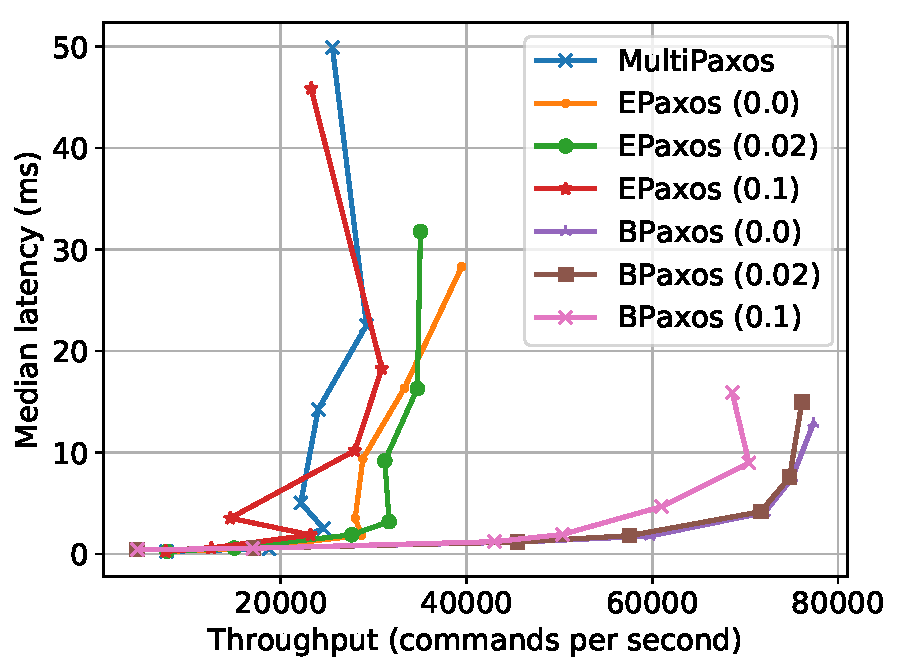
\includegraphics[width=\textwidth]{assets/nsdi_fig1_lt_f1.pdf}
    \caption{
      Latency-throughput curves for Multipaxos, EPaxos, and BPaxos. EPaxos and
      BPaxos are run with 0\%, 2\% and 10\% conflict rates. Here, $f = 1$.
    }\figlabel{EvalLtF1}
  \end{subfigure}
  \begin{subfigure}[c]{0.36\textwidth}
    \centering
    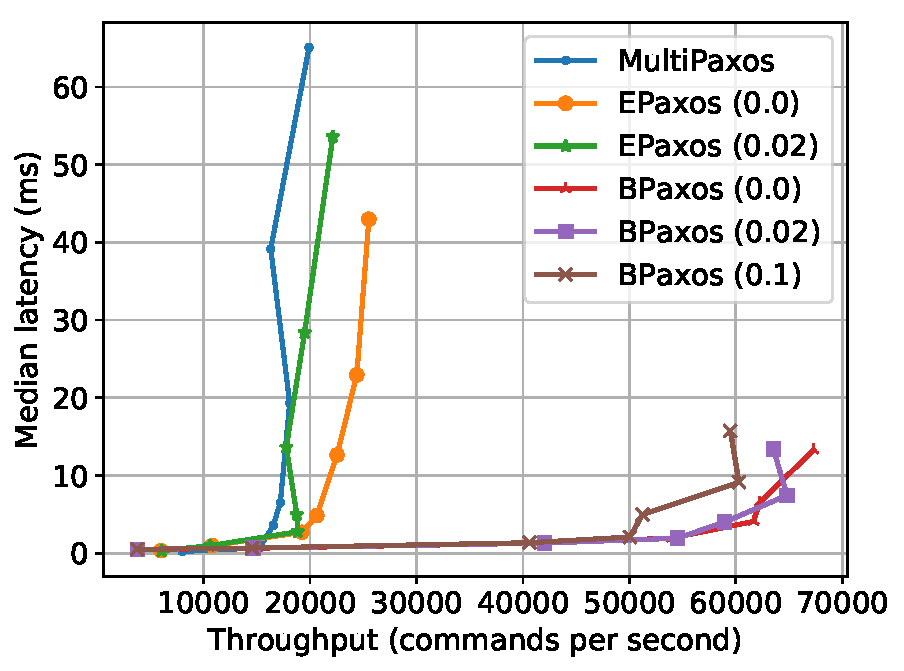
\includegraphics[width=\textwidth]{assets/nsdi_fig1_lt_f2.pdf}
    \caption{The same as \figref{EvalLtF1} but with $f=2$.}%
    \figlabel{EvalLtF2}
  \end{subfigure}
  \begin{subfigure}[c]{0.23\textwidth}
    \centering
    \small
    \begin{tabular}{lccc}
      \toprule
      \multicolumn{1}{c}{Protocol} &
      \multicolumn{3}{c}{Number of clients} \\
      %
                    & 1    & 10   & 50 \\\midrule
      Multipaxos    & 0.24 & 0.52 & 2.49 \\
      EPaxos (0.0)  & 0.25 & 0.56 & 1.83 \\
      EPaxos (0.02) & 0.25 & 0.57 & 1.89 \\
      EPaxos (0.1)  & 0.25 & 0.58 & 1.87 \\
      BPaxos (0.0)  & 0.41 & 0.56 & 1.16 \\
      BPaxos (0.02) & 0.41 & 0.56 & 1.17 \\
      BPaxos (0.1)  & 0.41 & 0.55 & 1.21 \\
      \bottomrule
    \end{tabular}
    \caption{%
      Median latency values (ms) from \figref{EvalLtF1}.
    }\figlabel{EvalLtTable}
  \end{subfigure}
  \caption{%
    Latency and throughput of Multipaxos, EPaxos, and BPaxos for varying number
    of clients, conflict rates, and values of $f$. Data is shown for $1$, $10$,
    $50$, $100$, $300$, $600$, and $1200$ clients.
  }\figlabel{EvalLt}
\end{figure*}
}

\paragraph{Experiment Description.}
We implemented MultiPaxos, EPaxos\footnote{%
  Note that we implement \emph{Basic} EPaxos, the algorithm outlined
  in~\cite{moraru2013proof}. In general, Basic EPaxos has larger quorums and
  simpler recovery compared to the complete EPaxos protocol which is described
  in~\cite{moraru2013there}. For $f=1$ though, the performance of the two
  protocols is practically identical.
}, and BPaxos in Scala\footnote{%
  To mitigate the effects of JVM garbage collection on our experiments, we run
  our experiments with a large heap size of 32GB and run experiments for only a
  short amount of time.
}. Here, we measure the throughput and latency of the three protocols with
respect to three parameters: the number of clients, the conflict rate, and the
parameter $f$.

\begin{itemize}
  \item \textbf{Clients.}
    Clients propose commands in a closed loop. That is, after a client proposes
    a command, it waits to receive a response before proposing another command.
    We also run multiple clients in the same process, so deployments with a
    large number of clients (e.g., $1200$ clients) may use only a few client
    processes. We run $1$, $10$, $50$, $100$, $300$, $600$, and $1200$ clients.

  \item \textbf{Conflict rate.}
    The protocols replicate a key-value store state machine. Commands are
    single key gets or single key sets. With a conflict rate of $r$, $r$ of the
    commands are sets to a single key, while $(1 - r)$ of the commands are gets
    to other keys. Keys and values are both eight bytes. If commands are large,
    the data path and control path can be split, as in~\cite{biely2012s}. We
    run with $r=0$, $r=0.02$, and $r=0.1$. As described
    in~\cite{moraru2013there}, workloads in practice often have very low
    conflict rates.

  \item \textbf{$f$.}
    Recall that a protocol with parameter $f$ must tolerate at most $f$ failures.
    We run with $f=1$ and $f=2$.
\end{itemize}

We deploy the three protocols on m5.4xlarge EC2 instances within a single
availability zone. MultiPaxos deploys $f+1$ proposers and $2f+1$ acceptors.
EPaxos deploys $2f+1$ replicas. BPaxos deploys $2f+1$ dependency service nodes,
$2f+1$ acceptors, $f+1$ replicas, $5$ leaders and proposers when $f=1$, and
$10$ leaders and proposers when $f=2$. Every logical node is deployed on its
own physical machine, except that every BPaxos leader is co-located with a
BPaxos proposer. The protocols do not perform batching. All three protocols
implement thriftiness, a standard optimization~\cite{moraru2013there}.

% no batching, execpt for graph execution
% thriftiness enabled
% num leaders for experiments
% m5.4xlarge machines in a single availability zone
% key value store with small keys and values, big keys do s-paxos
% clients not all different procs
% explain conflict rate (cite EPaxos saying conflict rates low)
% machine placement
% mention basic epaxos

\paragraph{Results.}
The benchmark results are shown in \figref{EvalLt}. In \figref{EvalLtF1} with
$f=1$, we see that MultiPaxos achieves a peak throughput of roughly 25,000 to
30,000 commands per second. EPaxos achieves a peak throughput of 30,000 to
40,000 depending on the conflict rate. BPaxos achieves 70,000 to 75,000,
nearly double that of EPaxos. Both EPaxos' and BPaxos' throughput decrease with
higher conflict rate. Higher conflict rates lead to graphs with more edges,
which increases the time required to topologically sort the graphs.

Note that the EPaxos implementation in~\cite{moraru2013there} achieves a peak
throughput of 45,000 to 50,000, slightly higher than our implementation. We
believe the discrepancy is due to implementation language (Go vs Scala) and
various optimizations performed in~\cite{moraru2013there} that we have not
implemented (e.g., a custom marshaling and RPC compiler~\cite{epaxos2019blog}).
We believe that if we apply the same optimizations to our implementations, all
three protocols' throughput would increase similarly.

In \figref{EvalLtF2}, with $f=2$, MultiPaxos' peak throughput has decreased to
20,000, EPaxos' peak throughput has decreased to 25,000, and BPaxos' peak
throughput has decreased to 65,000. As $f$ increases, the MultiPaxos leader has
to contact more nodes, so the drop in throughput is expected. With $f=2$,
EPaxos and BPaxos both have more leaders. More leaders increases the likelihood
of cycles, which slows the protocols down slightly. Moreover, when performing
dependency compaction as described in \secref{PracticalConsiderations}, the
number of dependencies scales with the number of leaders. BPaxos's peak
throughput is still roughly double that of EPaxos.

After sending a command, a BPaxos client must wait eight network delays to
receive a response. MultiPaxos and EPaxos require only four. Thus, under low
load, MultiPaxos and EPaxos have lower latency than BPaxos. In
\figref{EvalLtTable}, we see that with a single client, MultiPaxos and EPaxos
have a latency of roughly 0.25 ms, whereas BPaxos has a latency of 0.41. Under
high load though, BPaxos achieves lower latency. With 10 clients, the latency
of the three protocols is roughly even, and with 50 clients, BPaxos's latency
has already dropped below that of the other two protocols. In \figref{EvalLtF1}
and \figref{EvalLtF2}, we see that under higher loads of 600 and 1200 clients,
BPaxos's latency can be two to six times lower than the other two protocols.

Note that our results are specific to our deployment within a single data
center. With a geo-replicated deployment, MultiPaxos and EPaxos would both
outperform BPaxos. In this scenario, minimizing network delays is essential for
high performance.
%
Also note that BPaxos uses more machines than MultiPaxos and EPaxos in
order to achieve higher throughput via disaggregation and scaling. This makes
BPaxos a poor fit in resource constrained environments.

\subsection{Ablation Study}
{\begin{figure*}[ht]
  \centering
  \begin{subfigure}[b]{0.3\textwidth}
    \centering
    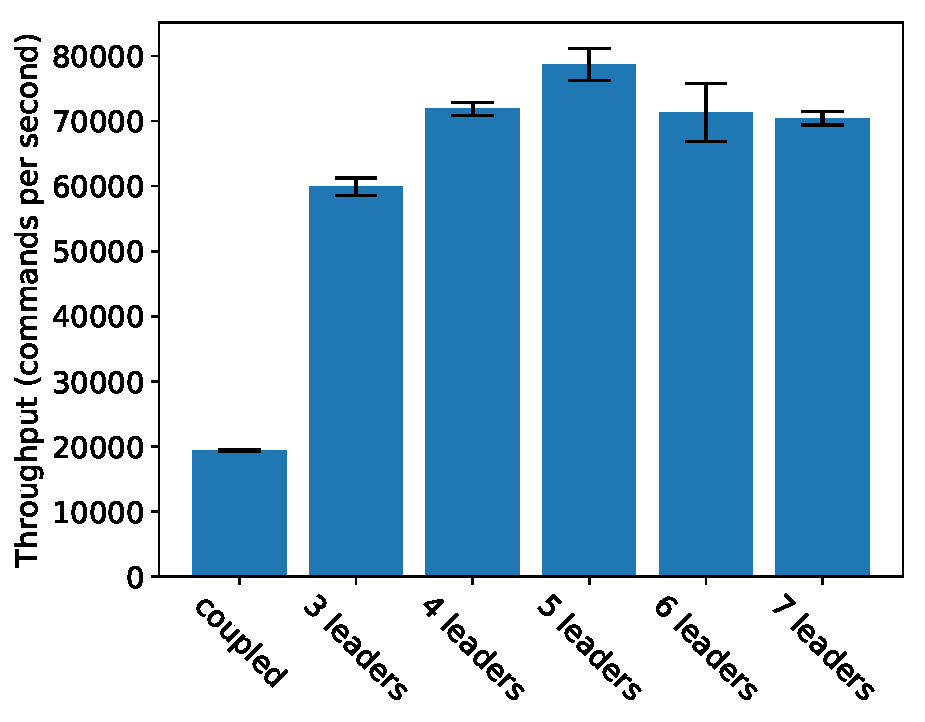
\includegraphics[width=\textwidth]{assets/nsdi_fig2_ablation_high_load_throughput.pdf}
    \caption{Throughput with 600 clients.}%
    \figlabel{EvalAblationHighLoadThroughput}
  \end{subfigure}\hspace{0.03\textwidth}
  \begin{subfigure}[b]{0.3\textwidth}
    \centering
    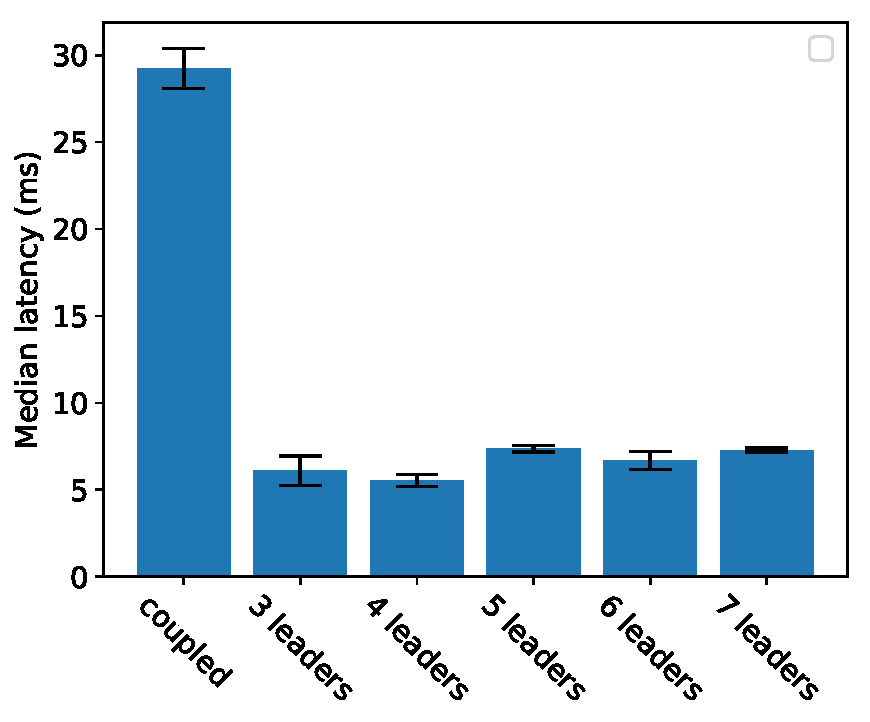
\includegraphics[width=\textwidth]{assets/nsdi_fig2_ablation_high_load_latency.pdf}
    \caption{Median latency (ms) with 600 clients.}%
    \figlabel{EvalAblationHighLoadLatency}
  \end{subfigure}\hspace{0.03\textwidth}
  \begin{subfigure}[b]{0.3\textwidth}
    \centering
    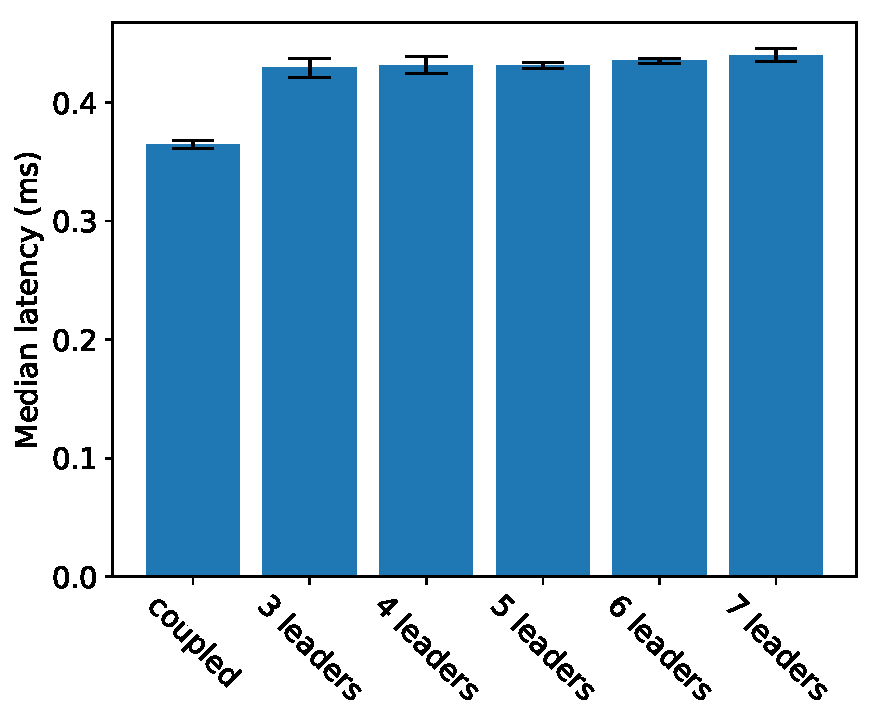
\includegraphics[width=\textwidth]{assets/nsdi_fig2_ablation_low_load_latency.pdf}
    \caption{Median latency (ms) with one client.}%
    \figlabel{EvalAblationLowLoadLatency}
  \end{subfigure}
  \caption{%
    An ablation study showing the effect of disaggregation and scaling on
    throughput and latency with 600 clients and one client. Throughput for one
    client is not shown because it is simply the inverse of latency.
  }\figlabel{EvalAblation}
\end{figure*}
}

\paragraph{Experiment Description.}
The previous experiment showed that BPaxos can achieve roughly double the
throughput of EPaxos. Now, we analyze how BPaxos achieves these speedups. In
particular, we perform an ablation study to measure how BPaxos' disaggregation
and scaling affect its throughput. We repeat the experiment from above with
$f=1$, with $r=0$, and with $1$ and $600$ clients. We vary the number of
leaders from $3$ to $7$. Moreover, we also consider a ``coupled BPaxos''
deployment with three machines where each machine runs a single process that
acts as a leader, a dependency service node, a proposer, an acceptor, and a
replica. This artificially coupled BPaxos is similar to EPaxos in which every
replica plays many roles.

% same setup as above
% run all components in one proc
% scale number of leaders
% see effects of decoupling and scaling
% high and low load

\paragraph{Results.}
The results of the experiment are shown in \figref{EvalAblation}. In
\figref{EvalAblationHighLoadThroughput}, we see the throughput of the coupled
BPaxos deployment is only 20,000 under high load. This is lower than both
MultiPaxos and EPaxos. When we decouple the protocol and run with three
leaders, the throughput increases threefold to 60,000. Disaggregating the nodes
introduces pipeline parallelism and reduces the load on the bottleneck
component. As we increase to five leaders, the throughput increases to a peak
of 75,000. At this point, the leaders are not the bottleneck and adding more
leaders only serves to slow down the protocol (for reasons similar to why the
$f=2$ deployment of BPaxos is slightly slower than the $f=1$ deployment).

In \figref{EvalAblationHighLoadLatency}, we see that the coupled protocol has
roughly six times the latency compared to the decoupled protocol under high
load. Moreover, the number of leaders doesn't have much of an impact on the
latency. In \figref{EvalAblationLowLoadLatency}, we see that the coupled
protocol has lower latency compared to the decoupled protocol under low load,
as fewer messages have to traverse the network. These results are consistent
with the previous experiment. Coupled protocols can achieve lower latency under
low load but decoupled protocols achieve higher throughput and lower latency
under high load.

In summary, both disaggregation and scaling contribute significantly to BPaxos'
increased throughput and lower latency under high load, and they also explain
why BPaxos has higher latency under low load.

% under high load, 600 clients, coupled perofrms worse than multipaxos and epaxos
% this is expected, bpaxos now has alot of orles
% when we doucple, we see triplign in throughput, already beating state of the art
% we scale up to 5 leaders to get an aditional 125\% throughput boost. once the leaders are not bottleneck, adding more doesnt help, it can acutallu hurt because more deps
%
% latency is helped by decoupling but leaders doest affect latency much
% at low load, the latency of coupled is slightly lower, fewer messages have to be sent across the network, this latency speedup would be even higher if we performened more aggresive forms of coupling
%
\subsection{Batching}
Existing state machine replication protocols can perform batching to increase
their throughput at the cost of some latency~\cite{santos2012tuning,
santos2013optimizing, moraru2013proof}. BPaxos uses decoupling and scaling to
increase throughput at the cost of some latency. These two techniques
accomplish the same goal but are orthogonal. We can add batching to BPaxos to
increase its throughput even further. BPaxos leaders can collect batches of
commands from clients and place all of them within a single vertex. While
batching improves the throughput of all replication protocols, BPaxos' modular
design enables the protocol to take advantage of batching particularly well.

First, the overheads of receiving client messages and forming batches falls
onto the leaders. Because we can scale the leaders, these overheads can be
amortized until they are no longer a bottleneck. Moreover, the execution time
of proposers and acceptors increases linearly with the number of batches, not
the number of commands. Thus, increasing the batch size also amortizes their
overheads. Finally, as batch sizes grow, the number of vertices and edges in
the replicas' graphs shrinks. Thus, replicas can topologically sort the smaller
graphs faster.

We repeated the benchmarks from above with $f=1$ and $r=0$ with a batch size of
$1000$ and achieved a peak throughput of roughly $500,000$ commands per second
with a median latency of roughly 200 ms.
}
{\section{Related Work}

\paragraph{Egalitarian Paxos}
Egalitarian Paxos, or EPaxos, is a leaderless consensus algorithm that aims to
achieve optimal commit latency and high throughput~\cite{moraru2013there,
moraru2013proof}. Many of the core ideas behind BPaxos were taken directly from
EPaxos. For example, EPaxos nodes construct directed graphs of commands and execute commands in reverse topological order one
strongly connected component at a time. BPaxos borrows this execution model
directly, formalizing it using notions of generalized consensus, dependency
graphs, eligible suffixes, and condensations.  EPaxos also maintains
\invref{ConsensusInvariant} and \invref{ConflictInvariant}, the two invariants
core to the BPaxos protocols.

However, EPaxos and the BPaxos protocols differ in the following ways.
%
First, EPaxos requires at least three message delays to commit a command,
whereas Unanimous BPaxos and Majority Commit BPaxos only require two (the
theoretical minimum).
%
Second, the BPaxos protocols considers a value $v$ chosen on the fast path
if there exists a fast quorum of acceptors that voted for $v$ in round $0$.
EPaxos, on the other hand, considers a value $v$ chosen on the fast path in
instance $I$ only if the leader of instance $I$ receives a fast quorum of votes
for $v$ in round $0$.  That is, in EPaxos, an instance's leader has the
ultimate authority on whether a value is chosen on the fast path.
%
Third, EPaxos has smaller fast quorums of size $f + \floor{\frac{f+1}{2}}$
compared to Majority Commit BPaxos' fast quorums of size $\SuperQuorumSize$.
%
Fourth, Majority Commit BPaxos considers a value $v = (x, \deps{I})$ chosen on
the fast path only if there exists some fast quorum $\FastQuorum$ of acceptors
that voted for $v$ in round $0$ and if for every $I' \in \deps{I}$, there
exists a quorum $\Quorum' \subseteq \FastQuorum$ of acceptors that know $I'$ is
chosen. EPaxos has a similar condition, but only requires that one acceptor in
$\FastQuorum$ know that $I'$ is chosen, rather than a quorum.

In summary, we can think of EPaxos as one protocol in the BPaxos family.
Compared to the BPaxos protocols presented in this paper, EPaxos has smaller
quorum sizes and more flexible conditions under which a value can be chosen on
the fast path. But, it has suboptimal commit latency and is less modular.

\paragraph{A Family of Leaderless Generalized Consensus Algorithms}
In~\cite{losa2016brief}, Losa et al.\ briefly announce a family of leaderless
generalized consensus algorithms. Losa et al.\ propose a generic generalized
consensus algorithm that is structured as the composition of a generic
dependency-set algorithm and a generic map-agreement algorithm. The invariants
of the dependency-set algorithm are essentially identical to
\invref{ConflictInvariant}, and the invariants of the map-agreement algorithm
are essentially identical to \invref{ConsensusInvariant}. Moreover, the example
implementations of these two algorithms given in~\cite{losa2016brief} form an
algorithm very similar to Simple BPaxos. Our paper builds on this body of work
by introducing Incorrect BPaxos, Unanimous BPaxos, Deadlock BPaxos, and
Majority Commit BPaxos.

\paragraph{Caesar}
Caesar~\cite{arun2017speeding} is a consensus algorithm that is very similar to
EPaxos and Majority Commit BPaxos. Caesar distinguishes itself by allowing a
command to be chosen on the fast path even if there does \emph{not} exist a
fast quorum of nodes that agree on the command's dependencies. Instead, Caesar
assigns timestamps to commands and only requires that a fast quorum of nodes
agree on a command's timestamp (as opposed to its dependencies). Doing so,
Caesar implements generalized consensus without maintaining
\invref{ConsensusInvariant}. Caesar achieves optimal commit latency and is
completely leaderless, but it is complicated by the fact that it does not
maintain \invref{ConsensusInvariant} and is not modular. As an interesting
avenue of future work, we would like to better understand the relationship
between Caesar and the BPaxos protocols.

\paragraph{Generalized Paxos and Variants}
Generalized Paxos~\cite{lamport2005generalized} exploits the commutativity of
state machine commands to reduce the number of conflicts that arise in
non-generalized consensus algorithms (e.g., Fast Paxos). Generalized Paxos has
optimal commit latency and is leaderless during normal processing, but when a
collision occurs (i.e., when acceptors disagree on the ordering of conflicting
commands), a distinguished leader is responsible for arbitrating collision
recovery. This leader becomes a bottleneck during recovery.
%
GPaxos~\cite{sutra2011fast} is a variant of Generalized Paxos that resolves
collisions with lower latency. Generalized Paxos requires at least four message
delays to recover a collision. GPaxos' two-step recovery requires at least two,
but still relies on a centralized leader. GPaxos' one-step recovery requires
only one message delay and distributes recovery among a set of acceptors.
However, GPaxos still increments the round number during recovery which affects
all commands, not just those that collided. The Bipartisan Paxos protocols
completely decouple the recovery of independent commands.

\paragraph{High Throughput Paxos Variants}
S-Paxos~\cite{biely2012s} is a Paxos variant that decouples control flow from
data flow. While S-Paxos still relies on a single leader for command ordering,
command dissemination is distributed across all nodes in the protocol. However,
S-Paxos does not achieve optimal commit latency and is not generalized.
%
Mencius~\cite{mao2008mencius} is a Multi-Paxos variant in which replicated log
entries are assigned round-robin to a set of leaders. This is in contrast to
Multi-Paxos where a single leader owns all of the log entries. However, Mencius
is not generalized. A leader may have to wait to hear from every other leader
before executing a command even if the command does not conflict with any other
command.

\paragraph{Other Paxos Variants}
Flexible Paxos~\cite{howard2016flexible} is a Paxos variant that takes
advantage of the fact that phase 1 and phase 2 quorums must intersect, but
phase 1 quorums do not have to intersect with other phase 1 quorums and phase 2
quorums do not have to intersect with other phase 2 quorums.
%
Speculative Paxos~\cite{ports2015designing} is a Paxos variant in which
replicas speculatively execute state machine commands before they are known to
be chosen. If commands are mostly ordered, then speculative execution can
improve performance.
%
We believe that flexible quorum sizes and speculative execution could both be
added to the BPaxos protocols to further improve their performance.
}
{\begin{figure*}[ht]
  \centering
  \tikzstyle{branch}=[draw, rounded corners, anchor=north, align=center,
                      fill=flatyellow!25]
  \tikzstyle{leaf}=[draw, anchor=north, align=left]
  \tikzstyle{edge}=[draw, thick, -latex]
  \tikzstyle{edgelabel}=[blue, inner sep=2pt, fill=white]
  \tikzstyle{highlight}=[draw=flatgreen, fill=flatgreen!5]
  \begin{tikzpicture}
    % Branches.
    \node[branch] (numLeaders) {number of\\leaders?};
    \node[branch] (generalizedLeft) at ($(numLeaders) + (200:3)$) {generalized?};
    \node[branch] (generalizedRight) at ($(numLeaders) + (-20:3)$) {generalized?};
    \node[branch] (commitTime) at ($(generalizedRight) + (-30:2)$) {commit\\time?};
    \node[branch] (tension) at ($(commitTime) + (-30:2.5)$) {tension\\handling?};

    % Leafs.
    \node[leaf] (paxos) at ($(generalizedLeft) + (210:2)$) {
      MultiPaxos~\cite{lamport1998part}\\
      Raft~\cite{ongaro2014search}\\
      VRR~\cite{liskov2012viewstamped}\\
      Chain Replication~\cite{van2004chain}
    };
    \node[leaf] (generalized) at ($(generalizedLeft) + (-30:2.2)$) {
      Generalized Paxos~\cite{lamport2005generalized}\\
      GPaxos~\cite{sutra2011fast}
    };
    \node[leaf] (mencius) at ($(generalizedRight) + (240:1.4)$) {
      Mencius~\cite{mao2008mencius}
    };
    \node[leaf, highlight] (simple) at ($(commitTime) + (210:2.5)$) {
      Simple \BPaxos{} (\S\ref{sec:SimpleBPaxos})
    };
    \node[leaf, highlight] (unanimous) at ($(tension) + (210:2.5)$) {
      Unanimous \BPaxos{} (\S\ref{sec:UnanimousBPaxos})\\
      Basic EPaxos~\cite{moraru2013there}\\
      Atlas~\cite{enes2020state}
    };
    \node[leaf, highlight] (majority) at ($(tension) + (-30:2.5)$) {
      Maj. Commit \BPaxos{} (\S\ref{sec:MajorityCommitBPaxos})\\
      EPaxos~\cite{moraru2013proof}\\
      Caesar~\cite{arun2017speeding}
    };

    % Edges.
    \draw[edge] (numLeaders) to node[edgelabel]{one} (generalizedLeft);
    \draw[edge] (numLeaders) to node[edgelabel]{many} (generalizedRight);
    \draw[edge] (generalizedLeft) to node[edgelabel]{no} (paxos);
    \draw[edge] (generalizedLeft) to node[edgelabel]{yes} (generalized);
    \draw[edge] (generalizedRight) to node[edgelabel]{no} (mencius);
    \draw[edge] (generalizedRight) to node[edgelabel]{yes} (commitTime);
    \draw[edge] (commitTime) to node[edgelabel]{$> 4$} (simple);
    \draw[edge] (commitTime) to node[edgelabel]{$\leq 4$} (tension);
    \draw[edge] (tension) to node[edgelabel]{avoiding} (unanimous);
    \draw[edge] (tension) to node[edgelabel]{resolving} (majority);
  \end{tikzpicture}

  \caption{%
    A non-exhaustive taxonomy of state machine replication protocols. The
    generalized multi-leader protocols that we discuss in this paper are shaded
    green.
  }
  \figlabel{Taxonomy}
\end{figure*}

\begin{table*}[ht]
  \centering
  \caption{%
    A summary of generalized multi-leader state machine replication
    protocols.
  }\tablabel{ProtocolSummary}%
  \begin{tabular}{llllllll}
    \toprule
                                                             &      & Commit & Tension    & Number of & Phase 1     & Classic Phase 2 & Fast Phase 2 \\
    Protocol                                                 & Safe & Time   & Handling   & Nodes     & Quorum Size & Quorum Size     & Quorum Size \\\midrule
    Simple \BPaxos{} (\S\ref{sec:SimpleBPaxos})              & yes  & 7      & N/A        & $2f+1$    & $f+1$       & $f+1$           & N/A \\
    Fast \BPaxos{} (\S\ref{sec:FastBPaxos})                  & no   & 4      & N/A        & $2f+1$    & $f+1$       & $f+1$           & $f+\maj{f+1}$  \\
    Unanimous \BPaxos{} (\S\ref{sec:UnanimousBPaxos})        & yes  & 4      & avoidance  & $2f+1$    & $f+1$       & $f+1$           & $2f+1$ \\
    Basic EPaxos~\cite{moraru2013there}                      & yes  & 4      & avoidance  & $2f+1$    & $f+1$       & $f+1$           & $2f$ \\
    Atlas~\cite{enes2020state}                               & yes  & 4      & avoidance  & $n$       & $f+1$       & $n-f$           & $\floor{\frac{n}{2}} + f$ \\
    Maj. Commit \BPaxos{} (\S\ref{sec:MajorityCommitBPaxos}) & yes  & 4      & resolution & $2f+1$    & $f+1$       & $f+1$           & $f + \maj{f+1}$ \\
    EPaxos~\cite{moraru2013proof}                            & yes  & 4      & resolution & $2f+1$    & $f+1$       & $f+1$           & $f + \maj{f+1} - 1$ \\
    Caesar~\cite{arun2017speeding}                           & yes  & 4      & resolution & $2f+1$    & $f+1$       & $f+1$           & $f + \maj{f+1}$ \\
    \bottomrule
  \end{tabular}
\end{table*}


\section{Conclusion}
In this paper, we explained, analyzed, and taxonomized generalized multi-leader
state machine replication protocols.
% Addresses Reviewer 1.
%
% > Figure 1 added little value to me. Except ``number of leaders'', terms in
% > other boxes are not yet defined. Also, it covers many protocols not
% > discussed in the paper.
\markrevisions{%
  Our taxonomy of state machine replication protocols is summarized in
  \figref{Taxonomy}, and a summary of the generalized multi-leader protocols
  that we discuss in this paper is given in \tabref{ProtocolSummary}.
}
%
We showed via Simple \BPaxos{} that simple generalized multi-leader protocols
do exist, but they have high commit time.  Reducing the commit time with Fast
\BPaxos{}, we discovered the fundamental tension between implementing consensus
and computing dependencies between commands. We taxonomized existing protocols
according to whether they avoid the tension (like Unanimous \BPaxos{}) or they
resolve the tension (like Majority Commit \BPaxos{}). Ultimately, we hope that
the clarity we have brought to the space can encourage more industry adoption
of generalized multi-leader protocols and can spur new academic innovations in
this space.
}

\bibliographystyle{plain}
\bibliography{references}

\appendix
{\onecolumn
\section{BPaxos TLA+ Specification}\applabel{TlaSpec}
\begin{verbatim}
------------------------------ MODULE SimpleBPaxos -----------------------------
(******************************************************************************)
(* This is a specification of Simple BPaxos. To keep things simple and to     *)
(* make models more easily checkable, we abstract a way a lot of the          *)
(* unimportant details of Simple BPaxos. In particular, the specification     *)
(* does not model messages being sent between components and does not         *)
(* include leaders, proposers, or replicas. The consensus service is also     *)
(* left abstract. The core of Simple BPaxos is that dependency service        *)
(* responses (noops) are proposed to a consensus service. This core of the    *)
(* algorithm is what is modelled.                                             *)
(*                                                                            *)
(* Run `tlc SimpleBPaxosModel` to check the model.                            *)
(******************************************************************************)

EXTENDS Dict, Integers, FiniteSets

(******************************************************************************)
(* Constants                                                                  *)
(******************************************************************************)

\* The set of commands that can be proposed to BPaxos. In this specification,
\* every command can be proposed at most once. This is mostly to keep behaviors
\* finite. In a real execution of Simple BPaxos, a command can be proposed an
\* infinite number of times.
CONSTANT Command
ASSUME IsFiniteSet(Command)

\* The command conflict relation. Conflict is a symmetric relation over Command
\* such that two commands a and b conflict if (a, b) is in Conflict.
CONSTANT Conflict
ASSUME
    /\ Conflict \subseteq Command \X Command
    /\ \A ab \in Conflict : <<ab[2], ab[1]>> \in Conflict

\* We assume the existence of a special noop command that does not conflict
\* with any other command. Because noop is not in Command, it does not appear
\* in Conflict.
CONSTANT noop
ASSUME noop \notin Command

\* The set of dependency service nodes.
CONSTANT DepServiceNode
ASSUME IsFiniteSet(DepServiceNode)

\* The set of dependency service quorums. Every two quorums must interesct.
\* Typically, we deploy 2f + 1 dependency service replicas and let quorums be
\* sets of replicas of size f + 1.
CONSTANT DepServiceQuorum
ASSUME
    /\ \A Q \in DepServiceQuorum : Q \subseteq DepServiceNode
    /\ \A Q1, Q2 \in DepServiceQuorum : Q1 \intersect Q2 /= {}

--------------------------------------------------------------------------------

(******************************************************************************)
(* Variables and definitions.                                                 *)
(******************************************************************************)
\* In Simple BPaxos, vertex ids are of the form Q.i where Q is a leader and i is
\* a monotonically increasing id (intially zero). In this specification, we
\* don't even model Simple BPaxos nodes. So, we let instances be simple
\* integers. You might imagine we would say `VertexId == Nat`, but keeping
\* things finite helps TLC. Every command can be proposed at most once, so
\* allowing instances to range between 0 and |Command| works great.
VertexId == 0..Cardinality(Command)

\* A proposal is a command (or noop) and its dependencies.
Proposal == [cmd: Command \union {noop}, deps: SUBSET VertexId]

\* The proposal associated with noop. Noop doesn't conflict with any other
\* command, so its dependencies are always empty.
noopProposal == [cmd |-> noop, deps |-> {}]

\* A dependency graph is a directed graph where each vertex is labelled with an
\* vertex id and contains a command. We model the graph as a dictionary mapping
\* a vertex id to its command and dependencies.
DependencyGraph == Dict(VertexId, Proposal)

\* dependencyGraphs[d] is the dependency graph maintained on dependency
\* service node d.
VARIABLE dependencyGraphs

\* The next vertex id to assign to a proposed command. It is initially 0 and
\* incremented after every proposed command.
VARIABLE nextVertexId

\* A dictionary mapping vertex id to the command proposed with that vertex id.
VARIABLE proposedCommands

\* A dictionary mapping vertex id to the set of proposals proposed to the
\* consensus service in that instance.
VARIABLE proposals

\* A dictionary mapping vertex id to the proposal that was chosen by the
\* consensus service for that vertex id.
VARIABLE chosen

vars == <<
  dependencyGraphs,
  nextVertexId,
  proposedCommands,
  proposals,
  chosen
>>

TypeOk ==
  /\ dependencyGraphs \in Dict(DepServiceNode, DependencyGraph)
  /\ nextVertexId \in VertexId
  /\ proposedCommands \in Dict(VertexId, Command)
  /\ proposals \in Dict(VertexId, SUBSET Proposal)
  /\ chosen \in Dict(VertexId, Proposal)

--------------------------------------------------------------------------------

(******************************************************************************)
(* Actions.                                                                   *)
(******************************************************************************)

\* Propose a command `cmd` to Simple BPaxos. In a real implementation of Simple
\* BPaxos, a client would send the command to a leader, and the leader would
\* forward the command to the set of dependency service nodes. Here, we bypass
\* all that. The only thing to do here is to assign the command an instance and
\* make sure it hasn't already been proposed.
ProposeCommand(cmd) ==
  /\ cmd \notin Values(proposedCommands)
  /\ proposedCommands' = [proposedCommands EXCEPT ![nextVertexId] = cmd]
  /\ nextVertexId' = nextVertexId + 1
  /\ UNCHANGED <<dependencyGraphs, proposals, chosen>>

\* Given a dependency graph G and command cmd, return the set of vertices in G
\* that contain commands that conflict with cmd. For example, consider the
\* following dependency graph with commands b, c, and d in vertices v_b, v_c,
\* and v_d. If command a conflicts with c and d, then the dependencies of a are
\* v_c and v_d.
\*
\*                                 v_b     v_c
\*                                +---+   +---+
\*                                | b +---> c |
\*                                +-+-+   +---+
\*                                  |
\*                                +-v-+
\*                                | d |
\*                                +---+
\*                                 v_d
Dependencies(G, cmd) ==
  {v \in VertexId : G[v] /= NULL /\ <<cmd, G[v].cmd>> \in Conflict}

\* Here, dependency service node d processes a request in vertex v. Namely,
\* it adds v to its dependency graph (along with the command in
\* proposedCommands). Dependency service nodes also do not process a command
\* more than once. In a real Simple BPaxos implementation, the dependency
\* service node would receive a message from a leader and send dependencies
\* back to the leader. Also, a dependency service node could receive a request
\* from the leader more than once. We abstract all of this away.
DepServiceProcess(d, v) ==
  LET G == dependencyGraphs[d] IN
  /\ proposedCommands[v] /= NULL
  /\ G[v] = NULL
  /\ LET cmd == proposedCommands[v] IN
    /\ dependencyGraphs' = [dependencyGraphs EXCEPT ![d][v] =
                              [cmd |-> cmd, deps |-> Dependencies(G, cmd)]]
    /\ UNCHANGED <<nextVertexId, proposedCommands, proposals, chosen>>

\* Evalutes to whether a quorum of dependency service nodes have processed the
\* command in vertex v.
ExistsQuorumReply(Q, v) ==
  \A d \in Q : dependencyGraphs[d][v] /= NULL

\* Evaluates to the dependency service reply for vertex v from quorum Q of
\* dependency service nodes.
QuorumReply(Q, v) ==
  LET responses == {dependencyGraphs[d][v] : d \in Q} IN
  [cmd |-> (CHOOSE response \in responses : TRUE).cmd,
   deps |-> UNION {response.deps : response \in responses}]

\* Propose a noop gadget in vertex v to the consensus service. In a real
\* Simple BPaxos implementation, a proposer would propose a noop only
\* in some circumstances. In this model, we allow noops to be proposed at any
\* time.
ConsensusProposeNoop(v) ==
  /\ proposals' = [proposals EXCEPT ![v] = @ \union {noopProposal}]
  /\ UNCHANGED <<dependencyGraphs, nextVertexId, proposedCommands, chosen>>

\* Propose a dependency service reply in vertex v to the consensus service.
ConsensusPropose(v) ==
  \E Q \in DepServiceQuorum :
    /\ ExistsQuorumReply(Q, v)
    /\ proposals' = [proposals EXCEPT ![v] = @ \union {QuorumReply(Q, v)}]
    /\ UNCHANGED <<dependencyGraphs, nextVertexId, proposedCommands, chosen>>

\* Choose a value for vertex v.
ConsensusChoose(v) ==
  /\ proposals[v] /= {}
  /\ chosen[v] = NULL
  /\ chosen' = [chosen EXCEPT ![v] = CHOOSE g \in proposals[v] : TRUE]
  /\ UNCHANGED <<dependencyGraphs, nextVertexId, proposedCommands, proposals>>

--------------------------------------------------------------------------------

(******************************************************************************)
(* Specification.                                                             *)
(******************************************************************************)
Init ==
  /\ dependencyGraphs = [d \in DepServiceNode |-> [v \in VertexId |-> NULL]]
  /\ nextVertexId = 0
  /\ proposedCommands = [v \in VertexId |-> NULL]
  /\ proposals = [v \in VertexId |-> {}]
  /\ chosen = [v \in VertexId |-> NULL]

Next ==
  \/ \E cmd \in Command : ProposeCommand(cmd)
  \/ \E d \in DepServiceNode : \E v \in VertexId : DepServiceProcess(d, v)
  \/ \E v \in VertexId : ConsensusProposeNoop(v)
  \/ \E v \in VertexId : ConsensusPropose(v)
  \/ \E v \in VertexId : ConsensusChoose(v)

Spec == Init /\ [][Next]_vars

FairSpec == Spec /\ WF_vars(Next)

--------------------------------------------------------------------------------

(******************************************************************************)
(* Properties and Invariants.                                                 *)
(******************************************************************************)
\* The consensus service can choose at most command in any given instance.
ConsensusConsistency ==
  \A v \in VertexId :
    chosen[v] /= NULL => chosen'[v] = chosen[v]

AlwaysConsensusConsistency ==
  [][ConsensusConsistency]_vars

\* If two conflicting commands a and b yield dependencies deps(a) and deps(b)
\* from the dependency service, then a is in deps(b), or b is in deps(a), or
\* both.
DepServiceConflicts ==
  \A v1, v2 \in VertexId :
  \A Q1, Q2 \in DepServiceQuorum :
  IF v1 /= v2 /\ ExistsQuorumReply(Q1, v1) /\ ExistsQuorumReply(Q2, v2) THEN
     LET proposal1 == QuorumReply(Q1, v1)
         proposal2 == QuorumReply(Q2, v2) IN
     <<proposal1.cmd, proposal2.cmd>> \in Conflict =>
       v1 \in proposal2.deps \/ v2 \in proposal1.deps
  ELSE
    TRUE

\* Simple BPaxos should only choose proposed commands. This is inspired by [1].
\*
\* [1]: github.com/efficient/epaxos/blob/master/tla+/EgalitarianPaxos.tla
Nontriviality ==
  \A v \in VertexId :
    chosen[v] /= NULL =>
      \/ chosen[v].cmd \in Values(proposedCommands)
      \/ chosen[v].cmd = noop

\* If two conflicting commands a and b are chosen, then a is in deps(b), or b
\* is in deps(a), or both.
ChosenConflicts ==
  \A v1, v2 \in VertexId :
  IF v1 /= v2 /\ chosen[v1] /= NULL /\ chosen[v2] /= NULL THEN
    LET proposal1 == chosen[v1]
        proposal2 == chosen[v2] IN
     <<proposal1.cmd, proposal2.cmd>> \in Conflict =>
       v1 \in proposal2.deps \/ v2 \in proposal1.deps
  ELSE
    TRUE

\* True if every command is chosen.
EverythingChosen ==
  \A cmd \in Command :
    \E v \in VertexId :
      /\ chosen[v] /= NULL
      /\ chosen[v] = cmd

\* Fairness free theorem.
THEOREM
  Spec => /\ AlwaysConsensusConsistency
          /\ []DepServiceConflicts
          /\ []Nontriviality
          /\ []ChosenConflicts

\* True if no noops are chosen.
NoNoop ==
  ~ \E v \in VertexId :
    /\ chosen[v] /= NULL
    /\ chosen[v].cmd = noop

\* If no noops are chosen, then every command is chosen. This property is only
\* true for FairSpec.
NoNoopEverythingChosen ==
  []NoNoop => <>EverythingChosen

\* Fairness theorem.
THEOREM
  FairSpec => /\ AlwaysConsensusConsistency
              /\ []DepServiceConflicts
              /\ []Nontriviality
              /\ []ChosenConflicts
              /\ NoNoopEverythingChosen

================================================================================
\end{verbatim}
}
\end{document}
